\documentclass[landscape]{foils} 
\newif\ifpdf
\ifx\pdfoutput\undefined
\pdffalse % we are not running PDFLaTeX
\else
\pdfoutput=1 % we are running PDFLaTeX
\pdftrue
\fi

\ifpdf
\usepackage[pdftex]{graphicx}
\else
\usepackage{graphicx}
\fi

\ifpdf
\DeclareGraphicsExtensions{.pdf, .jpg, .tif, .png}
\else
\DeclareGraphicsExtensions{.eps, .jpg}
\fi

%\usepackage{pslatex}
\usepackage{tabularx,dcolumn, graphicx, amsfonts,amsmath}  
\usepackage[sectionbib]{natbib}
\bibliographystyle{apalike}
\usepackage{picinpar}
\usepackage{multirow}
\usepackage{rotating}
\usepackage{paralist} %compactenum
\setlength{\voffset}{-0.5in}
%\setlength{\hoffset}{-0.5in}
%\setlength{\textwidth}{10.5in}
\setlength{\textheight}{7in}
\setlength{\parindent}{0pt}
%\pagestyle{empty}
%\renewcommand{\baselinestretch}{2.0}
\DeclareMathSymbol{\expect}{\mathalpha}{AMSb}{'105}
\def\p{\rm p}
\def\pp{\rm P}
% this are commands that come with the color package
\usepackage{color}
\usepackage{fancyhdr}


\pagestyle{empty}
%define colors
\definecolor{mediumblue}{rgb}{0.0509,0.35,0.568}
\definecolor{blue}{rgb}{0.0109,0.15,0.468}
\definecolor{black}{rgb}{0.04,0.06,0.2}
\definecolor{darkblue}{rgb}{0.03,0.1,0.2}
\definecolor{darkgreen}{rgb}{0.03,0.5,0.2}
\definecolor{lightblue}{rgb}{0.85,0.9333,0.95}
\definecolor{lightblue2}{rgb}{0.270588, 0.45098, 0.701961}
\definecolor{white}{rgb}{1.0,1.0,1.0}
\definecolor{yellow}{rgb}{0.961,0.972,0.047}
\definecolor{red}{rgb}{0.9,0.1,0.1}
\definecolor{orange}{rgb}{1.0,0.4,0.0}
\definecolor{grey}{rgb}{0.5,0.5,0.5}
\definecolor{violet}{rgb}{0.619608, 0.286275, 0.631373}
\definecolor{mybackgroundcolor}{rgb}{1.0,1.0,1.0}

%\definecolor{light}{rgb}{.5,0.5,0.0}
\definecolor{light}{rgb}{.3,0.3,0.3}

% sets backgroundcolor for whole document 
\pagecolor{mybackgroundcolor}
% sets text color
%\color{black}
% see below for an example how to change just a few words
% using \textcolor{color}{text}

\font \courier=pcrb scaled 2000
\newcommand{\notetoself}[1]{{\textsf{\textsc{\color{red} #1}}}\\}

\newcommand{\answer}[1]{{\sf \color{red} #1}}

\usepackage{pdfpages}

\newcommand{\section}{\secdef \newsection\newsection}
%\renewcommand{\labelitemi}{\includegraphics[width=5mm]{images/bullet.pdf}}
\newcommand{\newsection}[1]{%
{
	\par\flushleft\large\sf\bfseries \vskip -2cm #1\\\rule[0.7\baselineskip]{\textwidth}{0.5mm}\par}}

\newcommand{\subsection}{\secdef \test\test}
\newcommand{\test}[1]{%
	{\par\flushleft\normalsize\sf\bfseries #1: }}
\newcommand{\M}{\mathcal{M}}
\newcommand{\prob}{{\rm Prob~}}
\def\showy#1{{\normalsize\sf\bfseries #1}}
\def\donotuse#1{}

\newcommand{\entrylabel}[1]{\mbox{#1}\hfil}
\newenvironment{entry}
	{\begin{list}{}%
		{\renewcommand{\makelabel}{\entrylabel}%
		\setlength{\labelwidth}{35pt}%
		\setlength{\leftmargin}{\labelwidth+\labelsep}%
	}%
	{\end{list}}}

\newcommand{\poltext}{{\copyright\ 2002--2010 by Paul O. Lewis -- Modified by  Mark Holder with permission from Paul Lewis}}

\newcommand{\pol}{{\footnotesize \poltext}}
\newcommand{\myBackground}{\begin{picture}(0,0)(0,0)  \put(-40,-70){\makebox(0,0)[l]{\includegraphics[width=33cm]{images/baby_blue.jpg}}} \end{picture}}
\newcommand{\myFooter}{}
%\begin{picture}(0,0)(0,0)
%	\put(0,-185){\pol}
%\end{picture}}
\newcommand{\myNewSlide}{\newpage\myFooter} % \myBackground}

\usepackage{bm}
\usepackage{ifsym}
\usepackage{mathrsfs}
\usepackage{url}
\usepackage{hyperref}
\hypersetup{backref,  linkcolor=blue, citecolor=black, colorlinks=true, hyperindex=true}

\usepackage{pdfpages}
\usepackage{bm}
\usepackage{ifsym}

\begin{document}

\myNewSlide
\huge 
Thanks to Paul Lewis, Joe Felsenstein, and Peter Beerli for slides.

\myNewSlide
\section*{Reasons phylogenetic inference might be wrong}
\Large
\begin{compactenum}
	\item Our data might be wrong (``garbage in garbage out'')
	\item {\em Systematic error} -- Our inference method might not be sophisticated enough
	\item \underline{{\em Random error}} -- We might not have enough data, so we are misled by sampling error.
\end{compactenum}

(or it could be some combination of these).

{Focus of this evening: {\bf How confident can we be in the trees/splits inferred by ML?}}

\myNewSlide
\begin{compactenum}
	\item Bootstrapping to assess repeatability;
	\item Putting $P$-values on trees:
	\begin{compactitem}
		\item KH Test, SH Test
		\item parametric bootstrapping,
	\end{compactitem}
	\item Brief lab on parametric bootstrapping.
	\item Continue the onslaught of testing methods
	\begin{compactitem}
		\item aLRT, aBayes,
		\item 1 - BP,
		\item AU,
		\item aBP
	\end{compactitem}
	\item Cartoon time!
\end{compactenum}

\myNewSlide
\section*{Some resources related to this talk}
A \href{http://www.mendeley.com/groups/1275263/confidence-on-phylogenetic-trees/}{Mendeley Group} of papers related to topology testing on trees.

A \url{http://phylo.bio.ku.edu/woodshole/} has the beginnings of an annotated bibliography on this literature. Really this is just a few cryptic notes now. It will get better.

Eventually those notes and associated code at:\\ {\normalsize \url{https://github.com/mtholder/TreeTopoTestingTalks} }


\myNewSlide
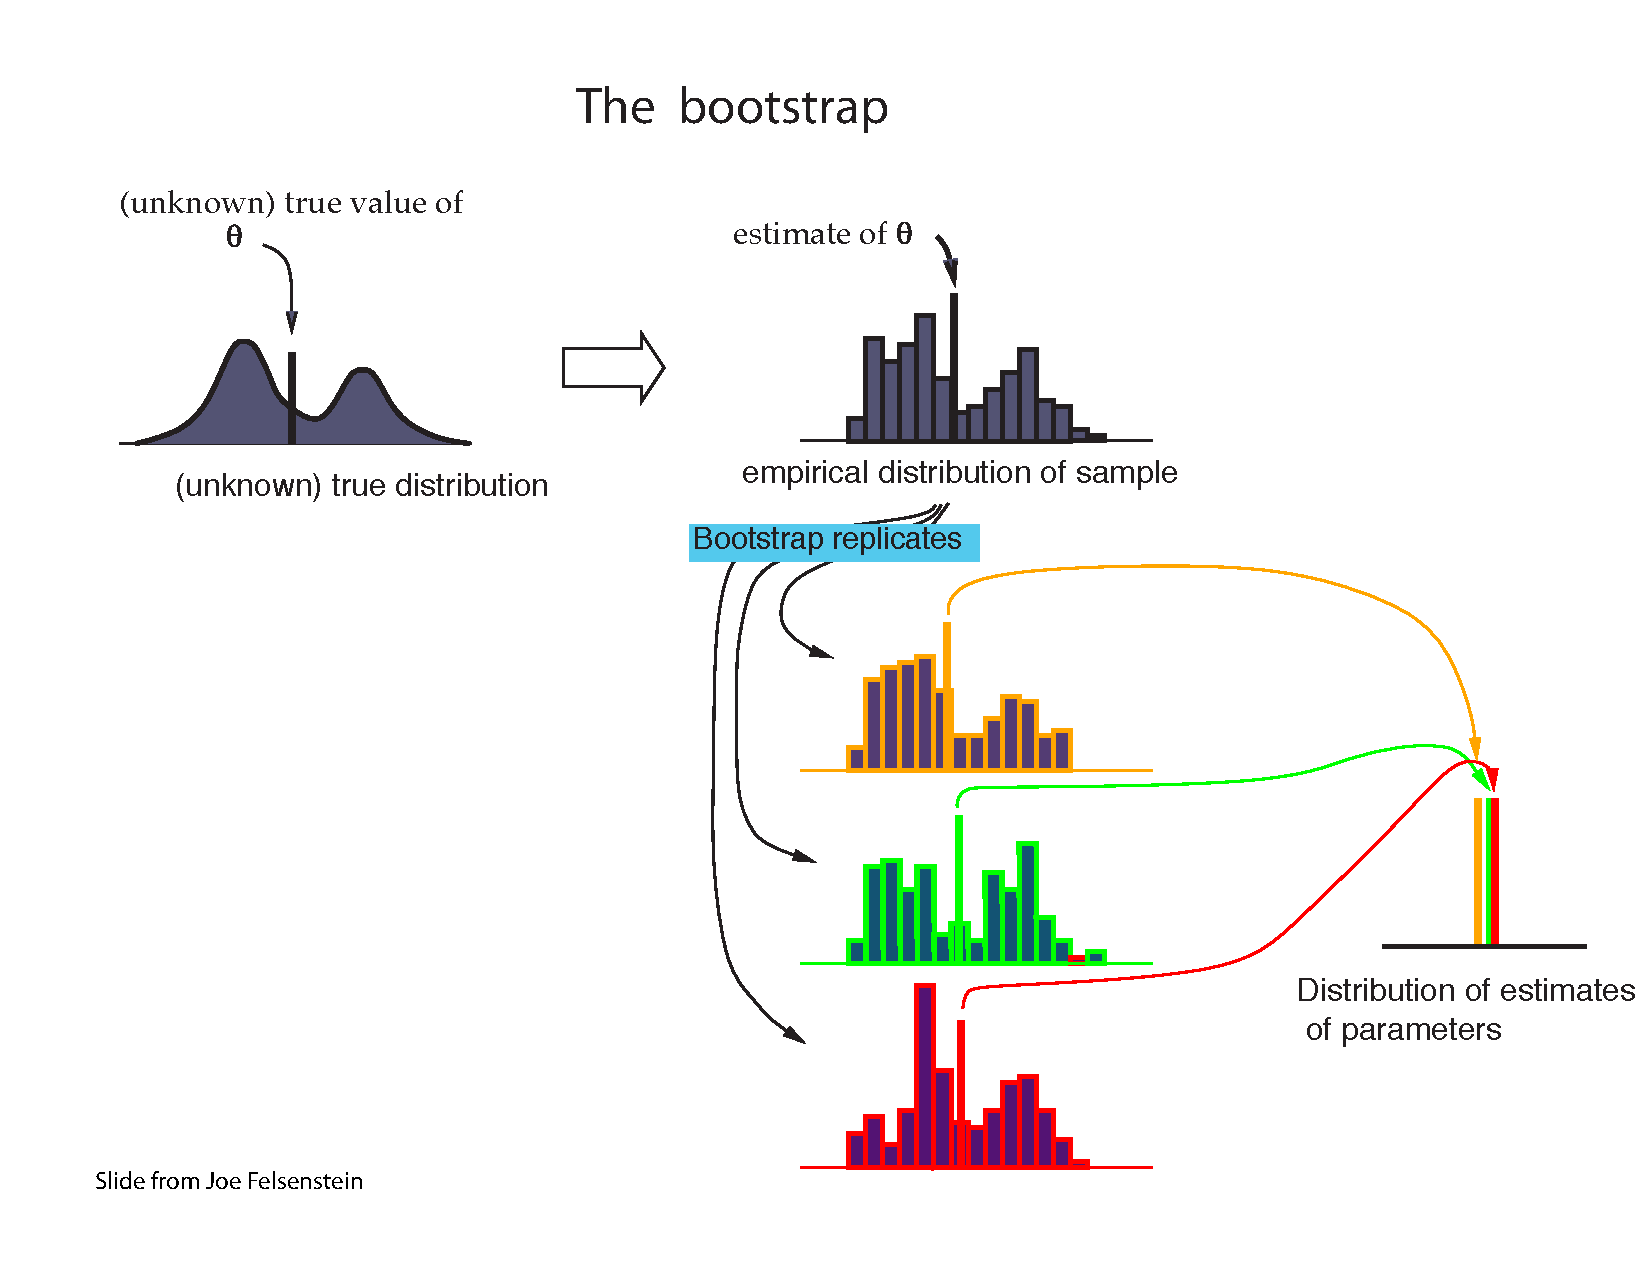
\includepdf[pages={1}]{../newimages/JoeFelsBootFig1.pdf} 

\myNewSlide
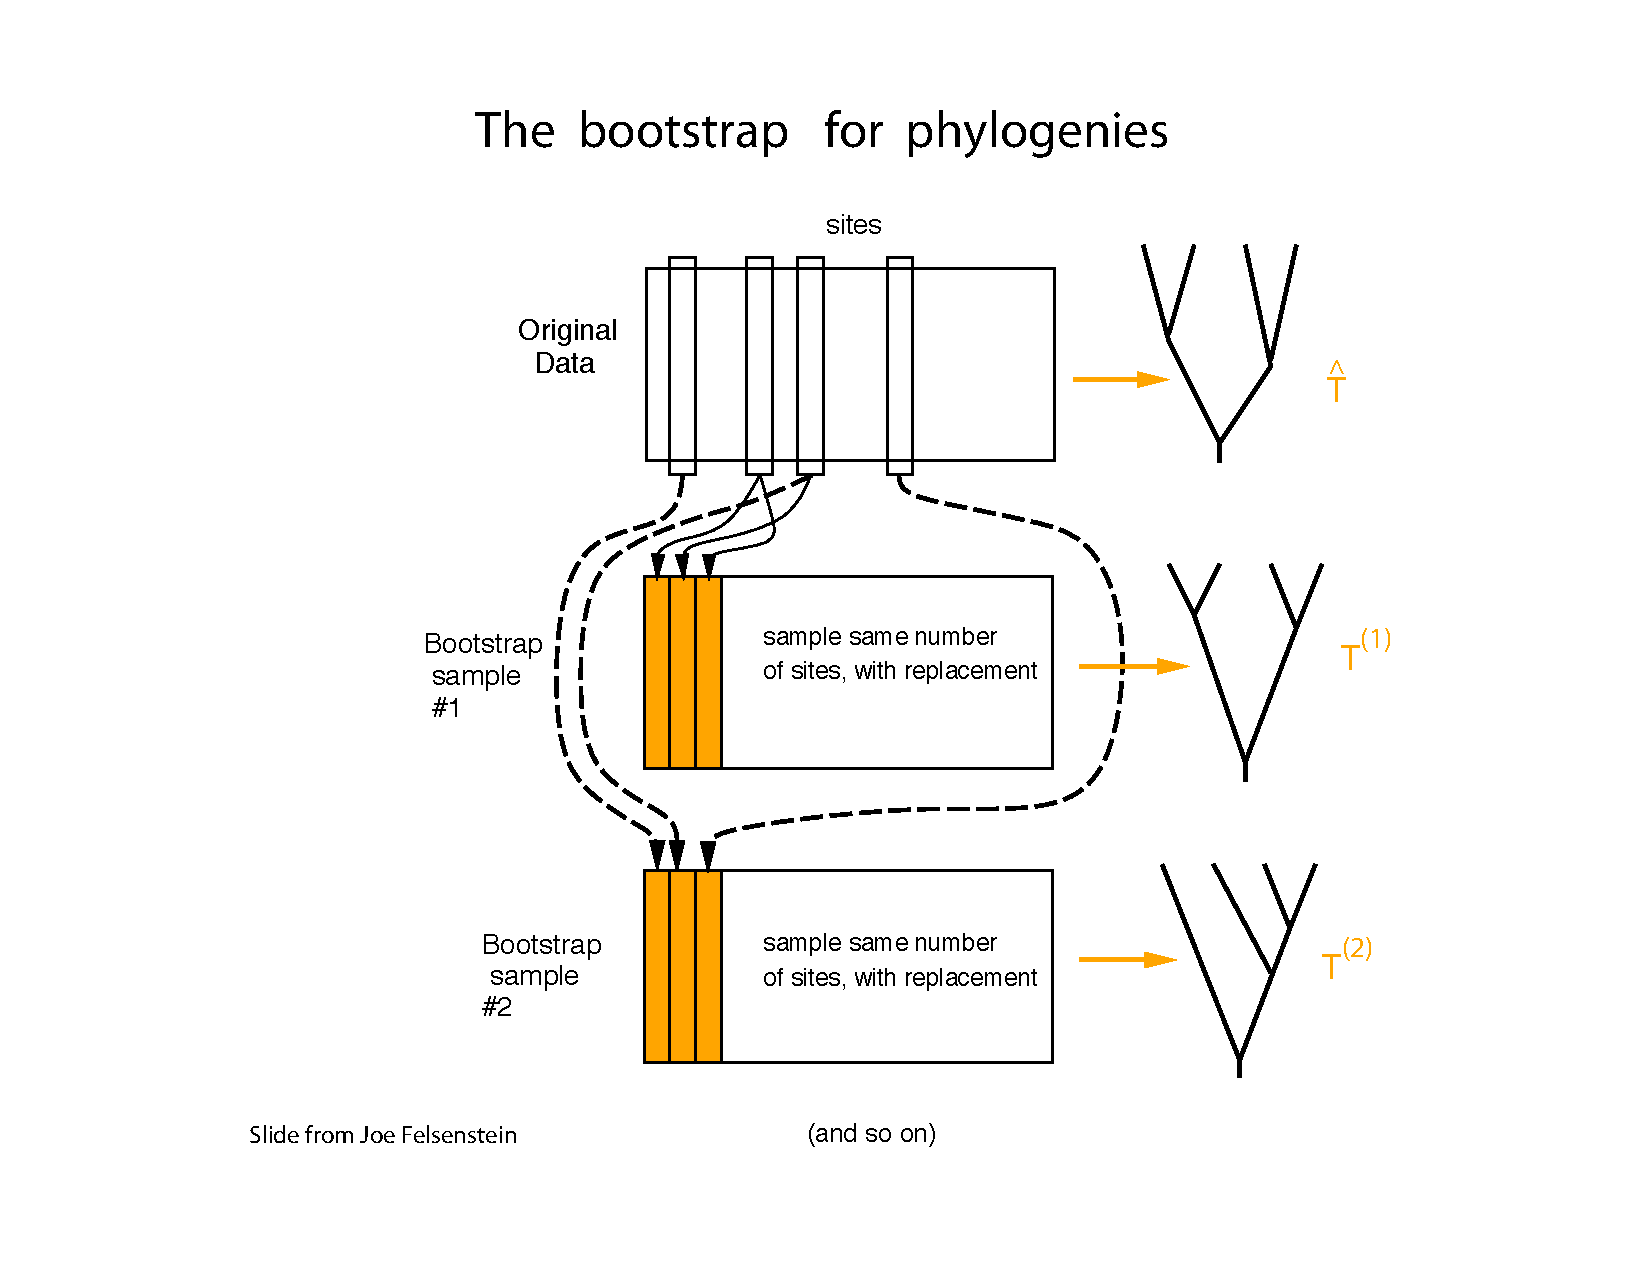
\includepdf[pages={1}]{../newimages/JoeFelsBootFig2.pdf} 

\myNewSlide
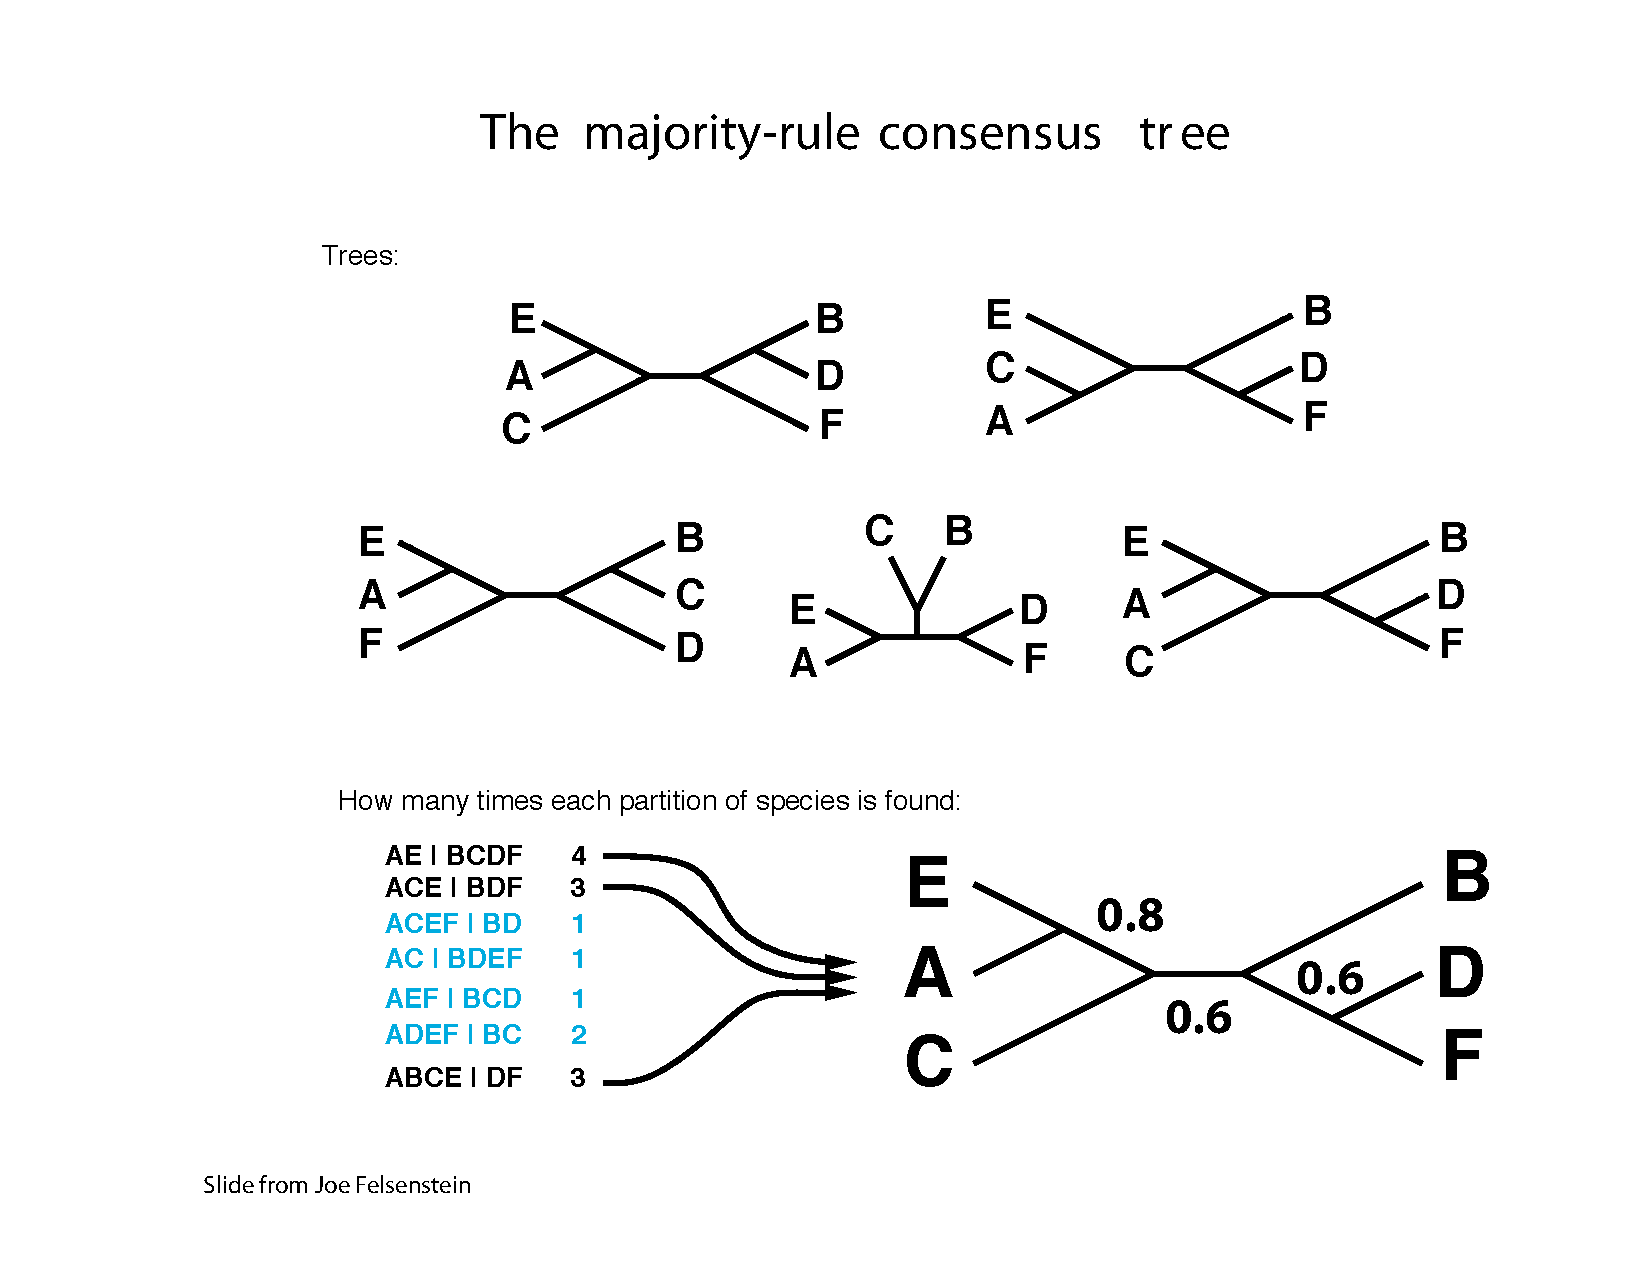
\includepdf[pages={1}]{../newimages/JoeFelsBootFig3.pdf} 

\myNewSlide
\begin{picture}(0,0)(0,0)
	  \put(0,-180){\makebox(0,0)[l]{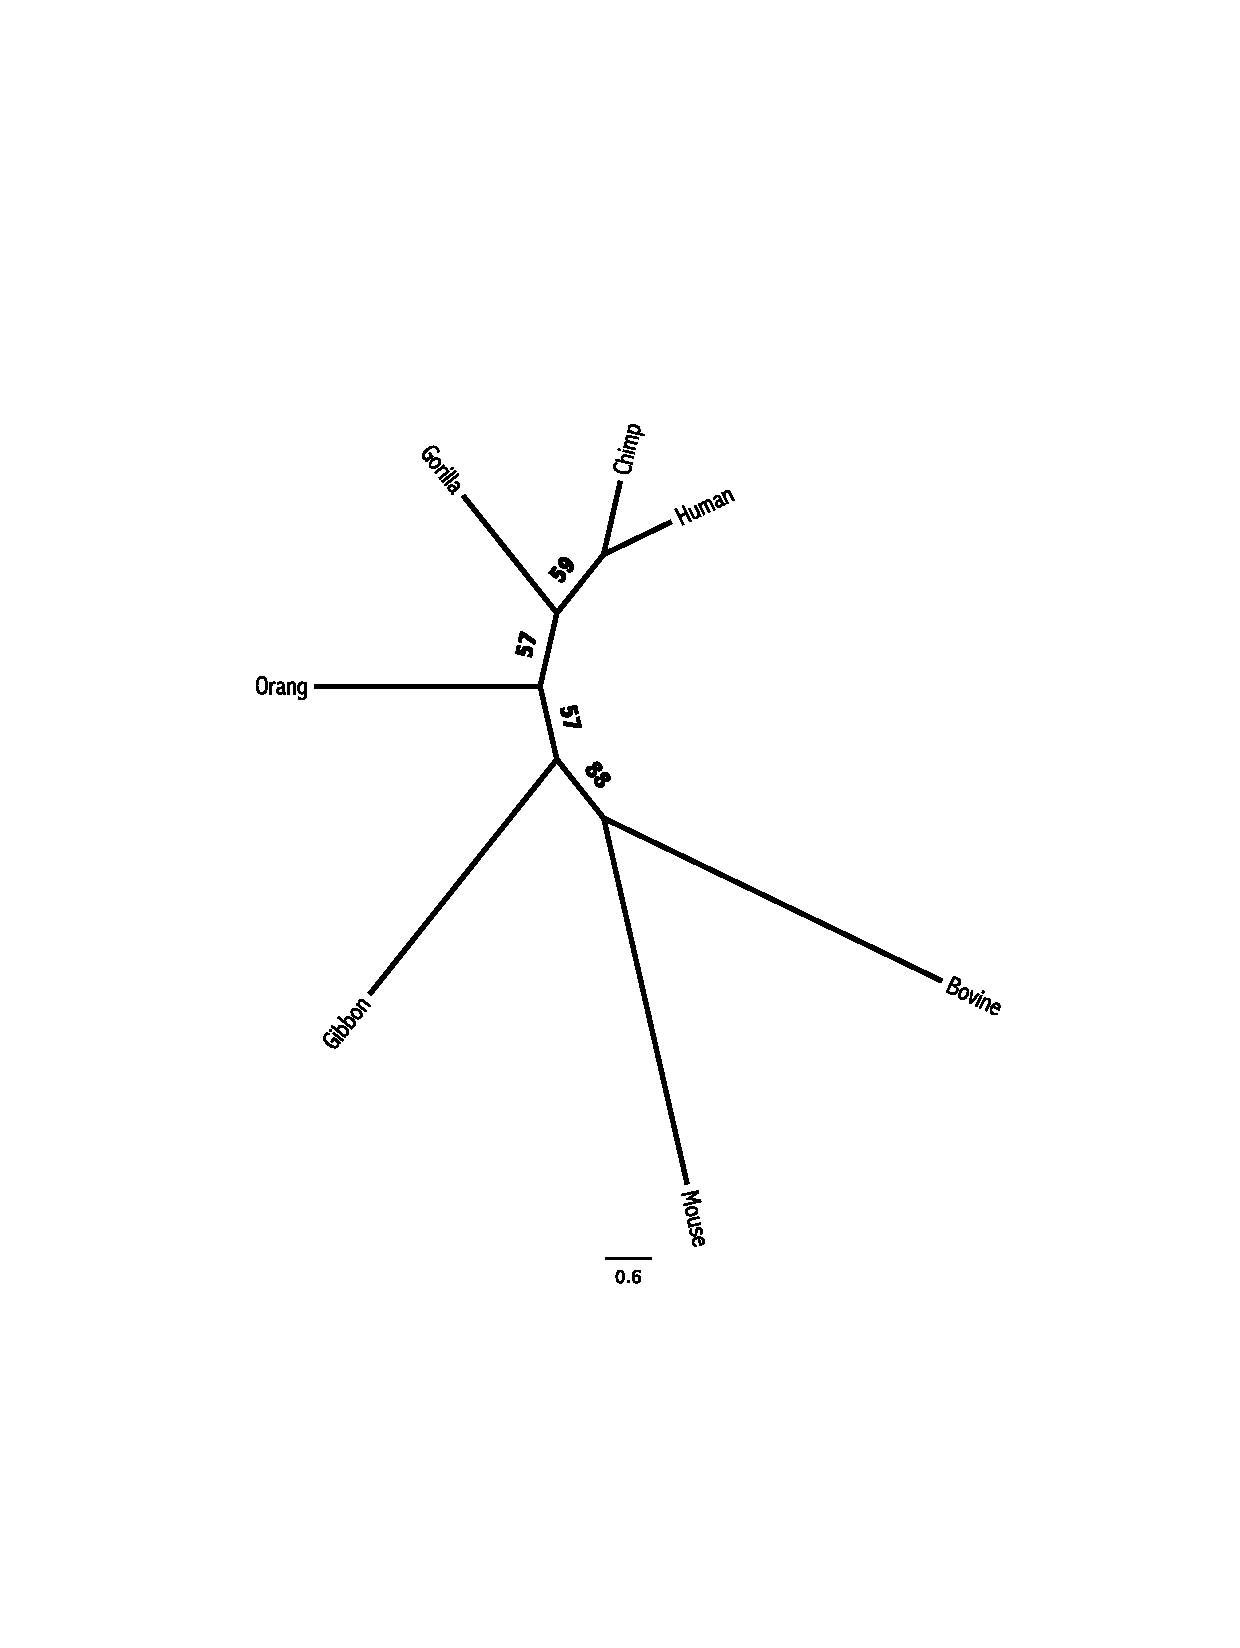
\includegraphics[scale=1.2]{../newimages/hasegawaBootFigTree.pdf}}}
	  \put(0,-350){\small From Hasegawa's analysis of 232 sites D-loop}
\end{picture}

\myNewSlide
\section*{Bootstrapping for branch support}
\large
\begin{itemize}
	\item ``Rogue'' taxa can lower support for many splits -- you do not have to use the majority-rule consensus tree to summarize bootstrap confidence statements.
	\item Less thorough searching is faster, but will usually artificially lower BP. However, \citet{AnisimovaGDDG2011} report that RAxML's rapid bootstrap algorithm may inflate bootstrap proportions).
\end{itemize}

\myNewSlide
\section*{Bootstrapping as a noisy measure of repeatability}
\begin{picture}(0,0)(0,0)
	  \put(0,-280){\makebox(0,0)[l]{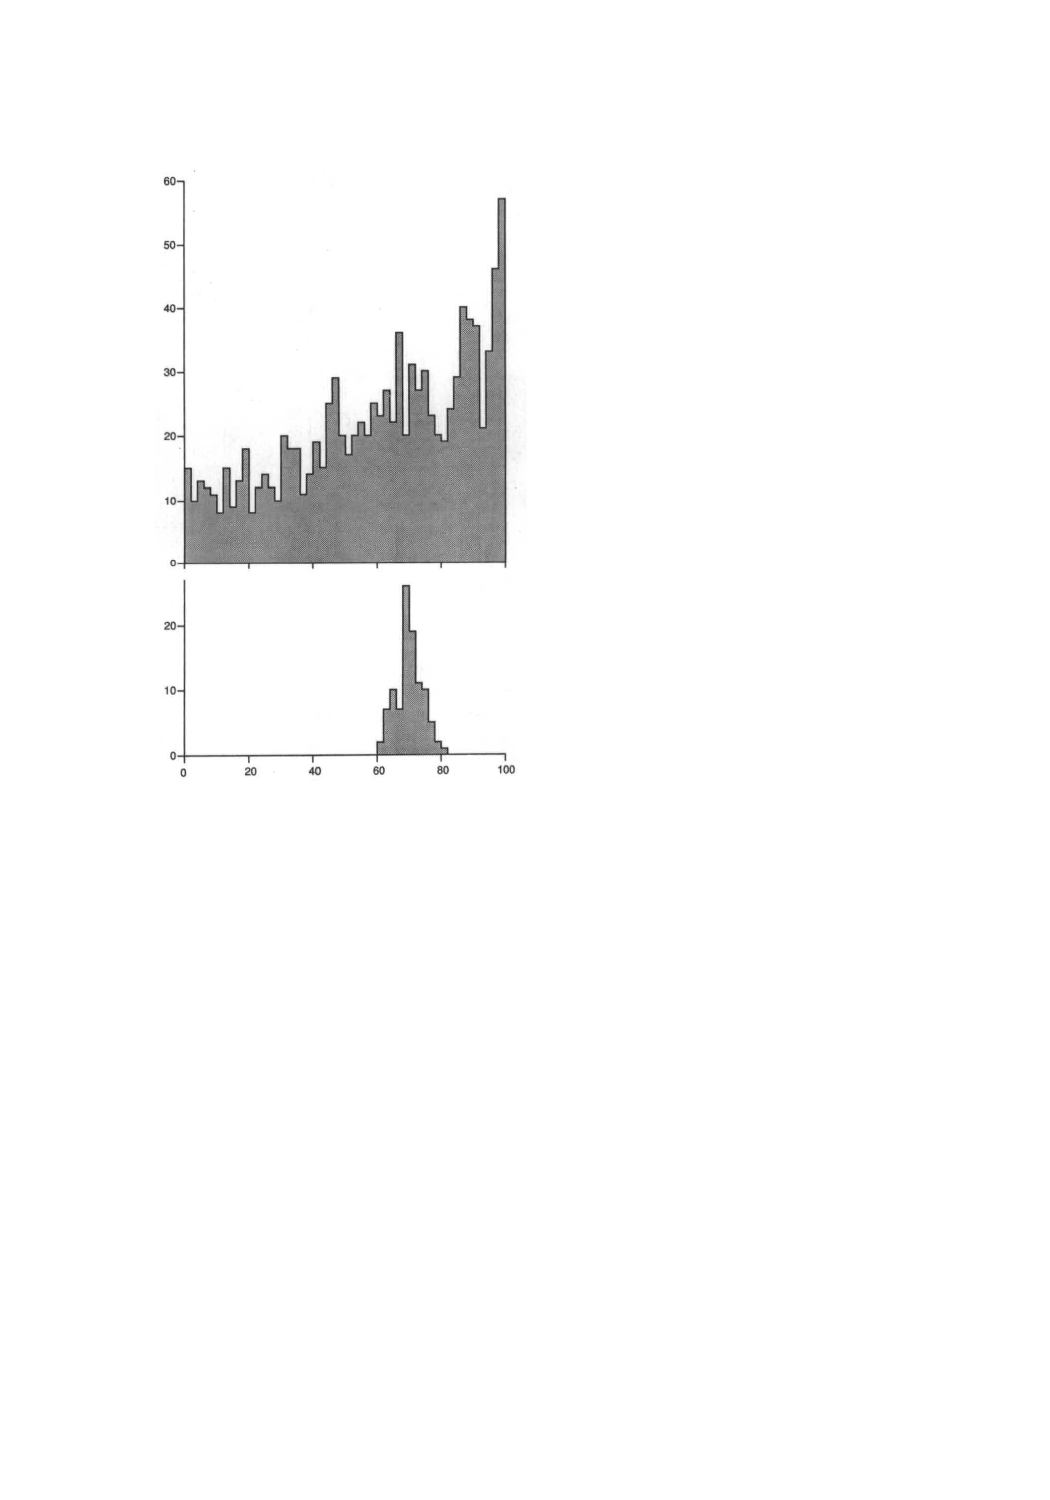
\includegraphics[scale=1.2]{../newimages/HillisB1993Fig3.pdf}}}
	  \put(150,-330){\small \% recovering tree}
	  \put(0,-20){\small repeated}
	  \put(0,-50){\small bootstrapping}
	  \put(0,-220){\small repeated}
	  \put(0,-250){\small simulation}
	  \put(350,-170){Simulation study of }
	  \put(350,-200){\citet{HillisB1993} }
\end{picture}


\myNewSlide
\section*{Frequentist hypothesis testing: coin flipping example}
$N=100$ and $h=60$\\
Can we reject the hypothesis of a fair coin ($p_H = 0.5$)?

The ``recipe'' is:
\begin{compactenum}
	\item Formulate null ($H_0$) and alternative ($H_A$) hypotheses.
	\item Choose an acceptable Type-I error rate.
	\item Choose a test statistic: $f_H$= fraction of heads in sample. $f_H=0.6$
	\item Identify the tail region of the test statistic - the values that conflict with $H_0$ at least a strongly as your observed data.
	\item Calculate the $P$-value: The probability of a test statistic value more extreme than $0.6$ arising {\em even if $H_0$  is true}.
	\item Reject $H_0$ if $P$-value is $\leq$ your Type I error rate.
\end{compactenum}

\myNewSlide
\begin{picture}(500,0)(0,0)
	  \put(0,-190){\makebox(0,0)[l]{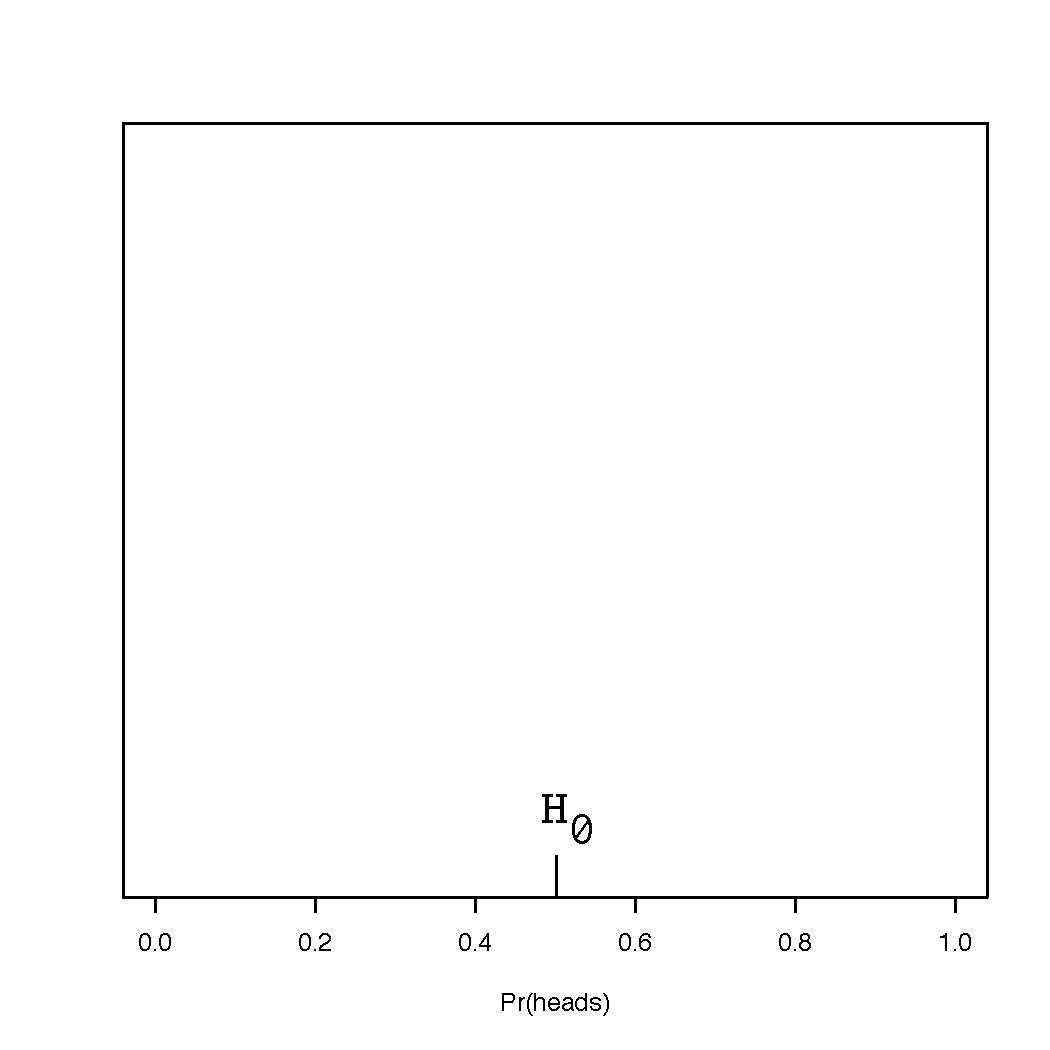
\includegraphics[scale=1.0]{../newimages/coin_axes.pdf}}}
\end{picture}

\myNewSlide
\begin{picture}(500,0)(0,0)
	  \put(0,-190){\makebox(0,0)[l]{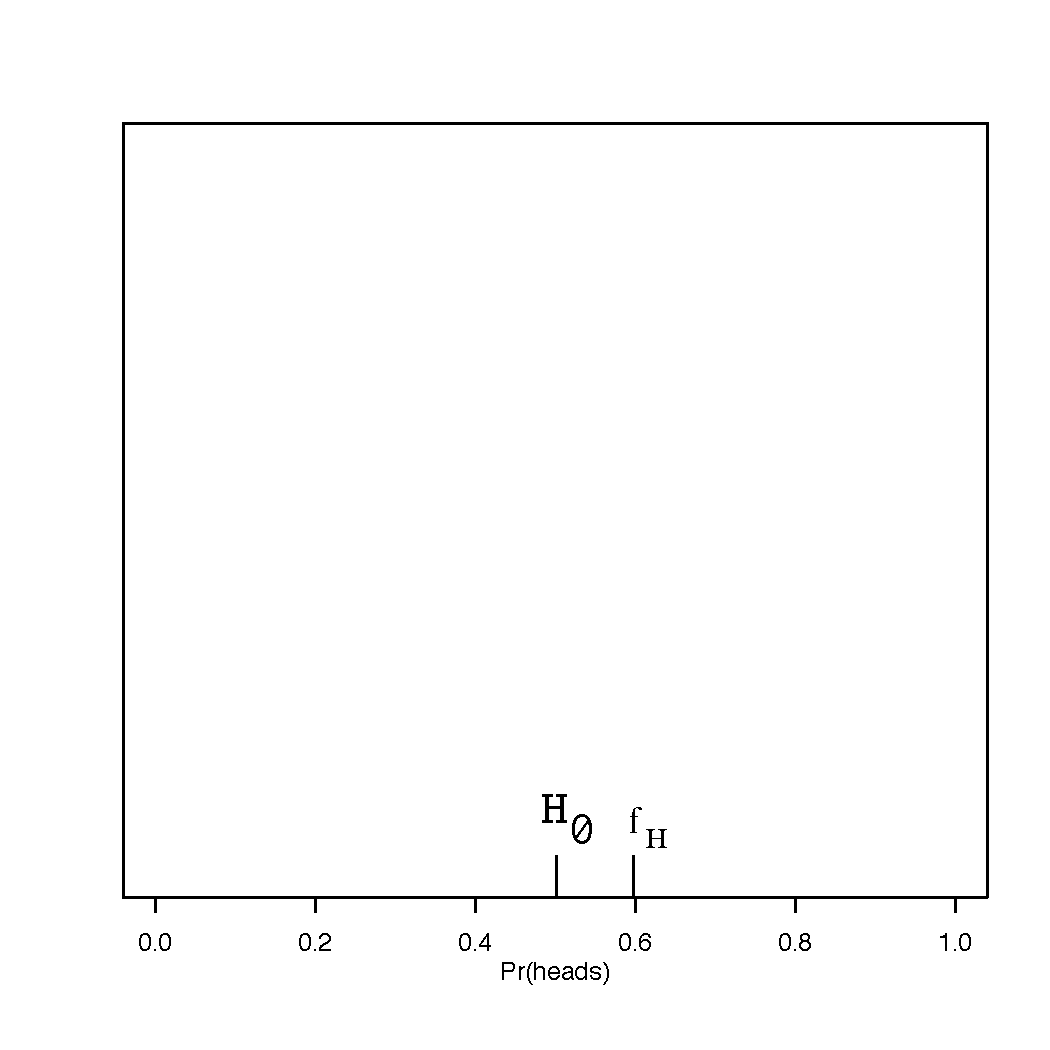
\includegraphics[scale=1.0]{../newimages/coin_axes_data.pdf}}}
\end{picture}

\myNewSlide
\begin{picture}(500,0)(0,0)
	  \put(0,-190){\makebox(0,0)[l]{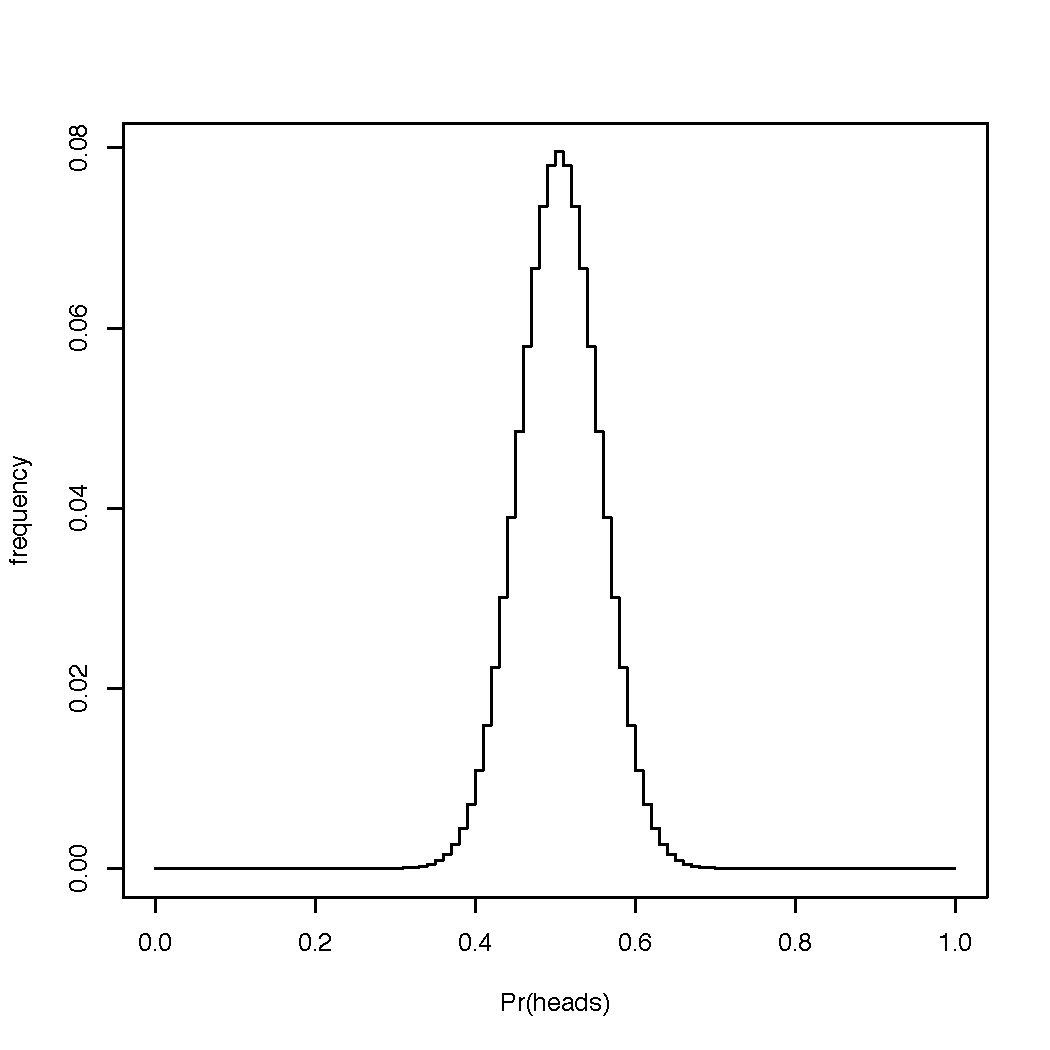
\includegraphics[scale=1.0]{../newimages/coin_wo_tails.pdf}}}
\end{picture}

\myNewSlide
\begin{picture}(500,0)(0,0)
	  \put(0,-190){\makebox(0,0)[l]{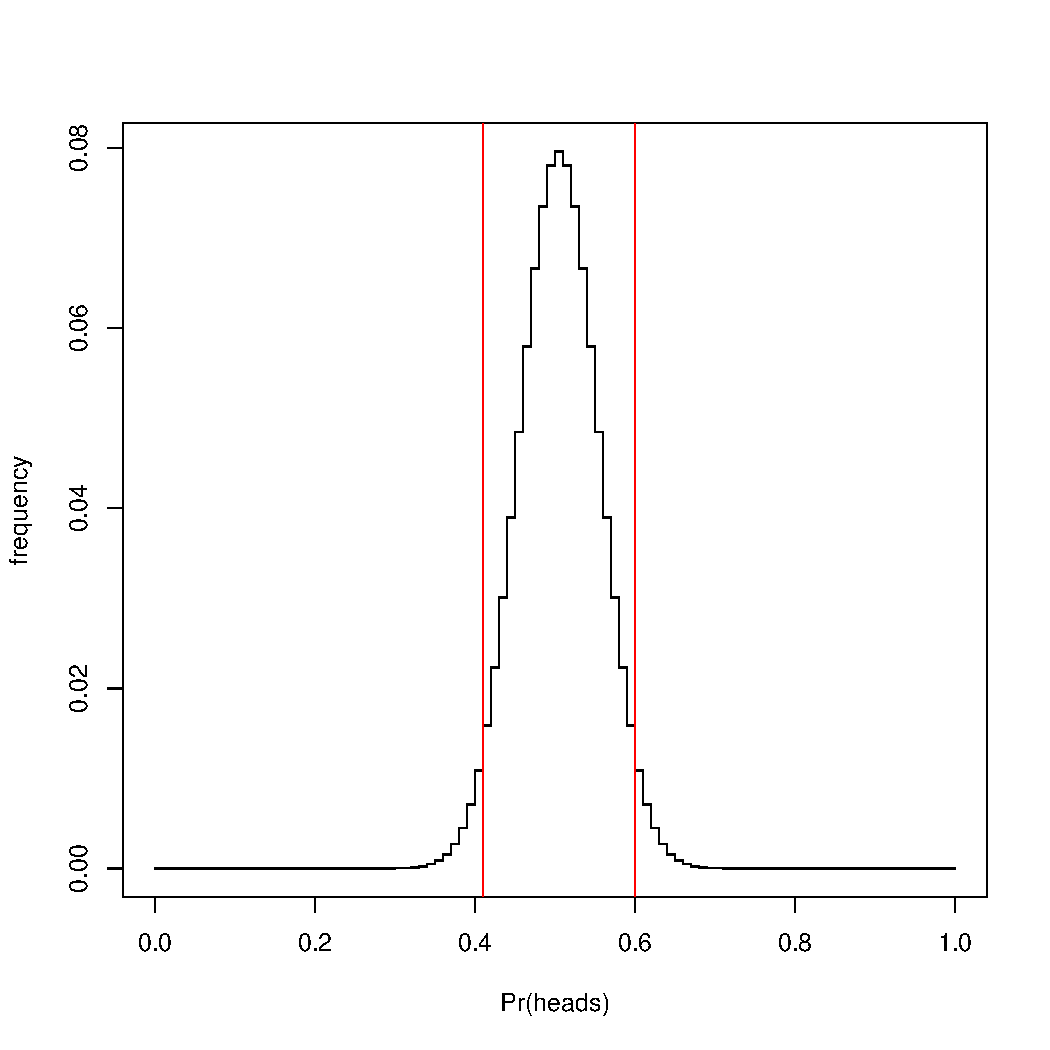
\includegraphics[scale=1.0]{../newimages/coin_w_tails.pdf}}}
	  \put(0,-450){$P$-value $\approx$ 0.058}
\end{picture}

\myNewSlide
Making similar plots for tree inference is hard.

Our parameter space is trees and branch lengths. Our data is a matrix of characters. It is hard to put these objects on the same plot.

We will see later (during ``cartoon time''), that we {\em can} visualize them both in a parameter space that describes how frequent different patterns of data are.


\myNewSlide
\section*{The simplest phylogenetic test would compare two trees}
\Large
Null: If we had no sampling error (infinite data) $T_1$ and $T_2$ would explain the data equally well. 

Test Statistic: $$\delta(T_1,T_2|X) = 2\left[\ln L(T_1|X) - \ln L(T_2|X)\right]$$

Expectation under null: $$\mathbb{E}_{H_0}\left[\delta(T_1,T_2|X)\right] = 0$$


\myNewSlide
\begin{picture}(500,0)(-20,-50)
	  \put(20,-20){\small Using 3000 sites of mtDNA sequence for 5 primates}
	  \put(20,-60){\normalsize $T_1$ is ((chimp, gorilla), human)}
	  \put(50,-200){\makebox(0,-190)[l]{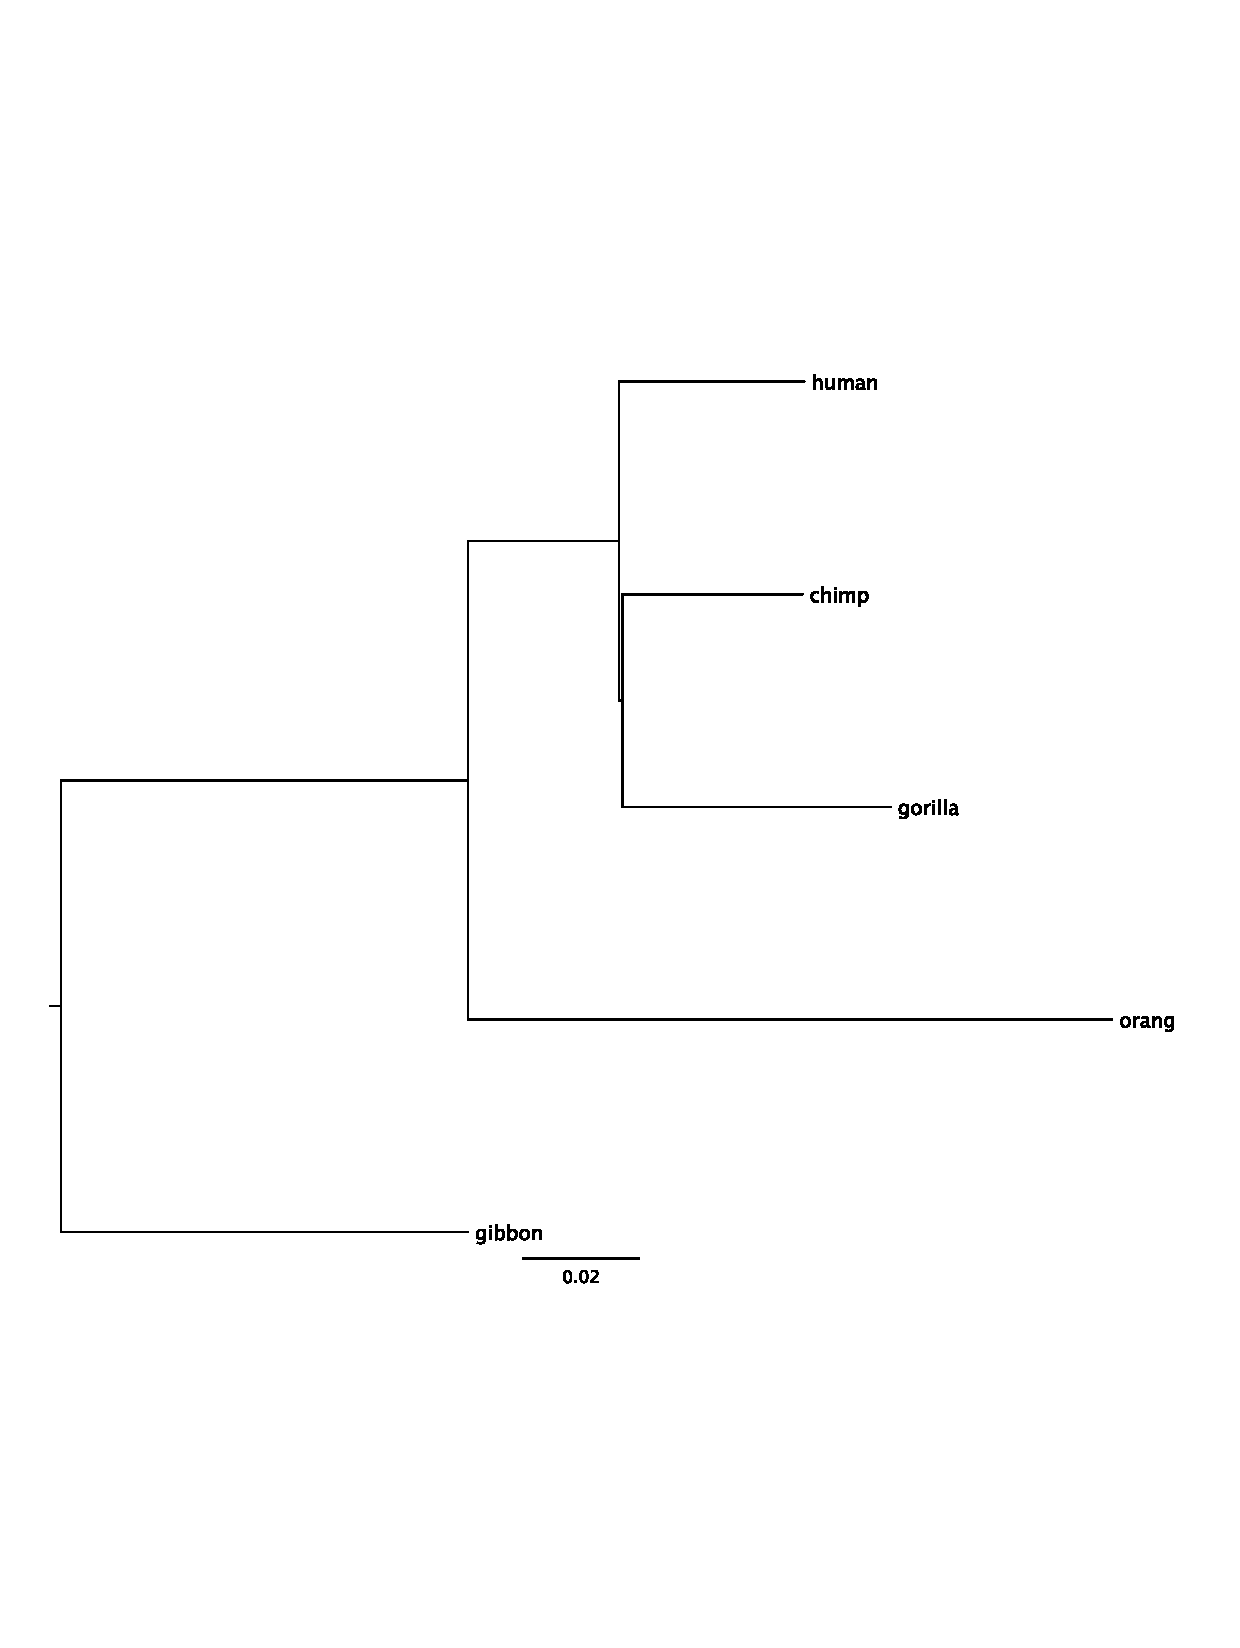
\includegraphics[scale=1.0]{../scripts/mtdna/chimpGorilla3000sites.pdf}}}
\end{picture}

\myNewSlide
\begin{picture}(500,0)(-20,-50)
	  \put(20,-20){\small Using 3000 sites of mtDNA sequence for 5 primates}
	  \put(20,-60){\normalsize $T_2$ is ((chimp, human), gorilla)}
	  \put(50,-200){\makebox(0,-190)[l]{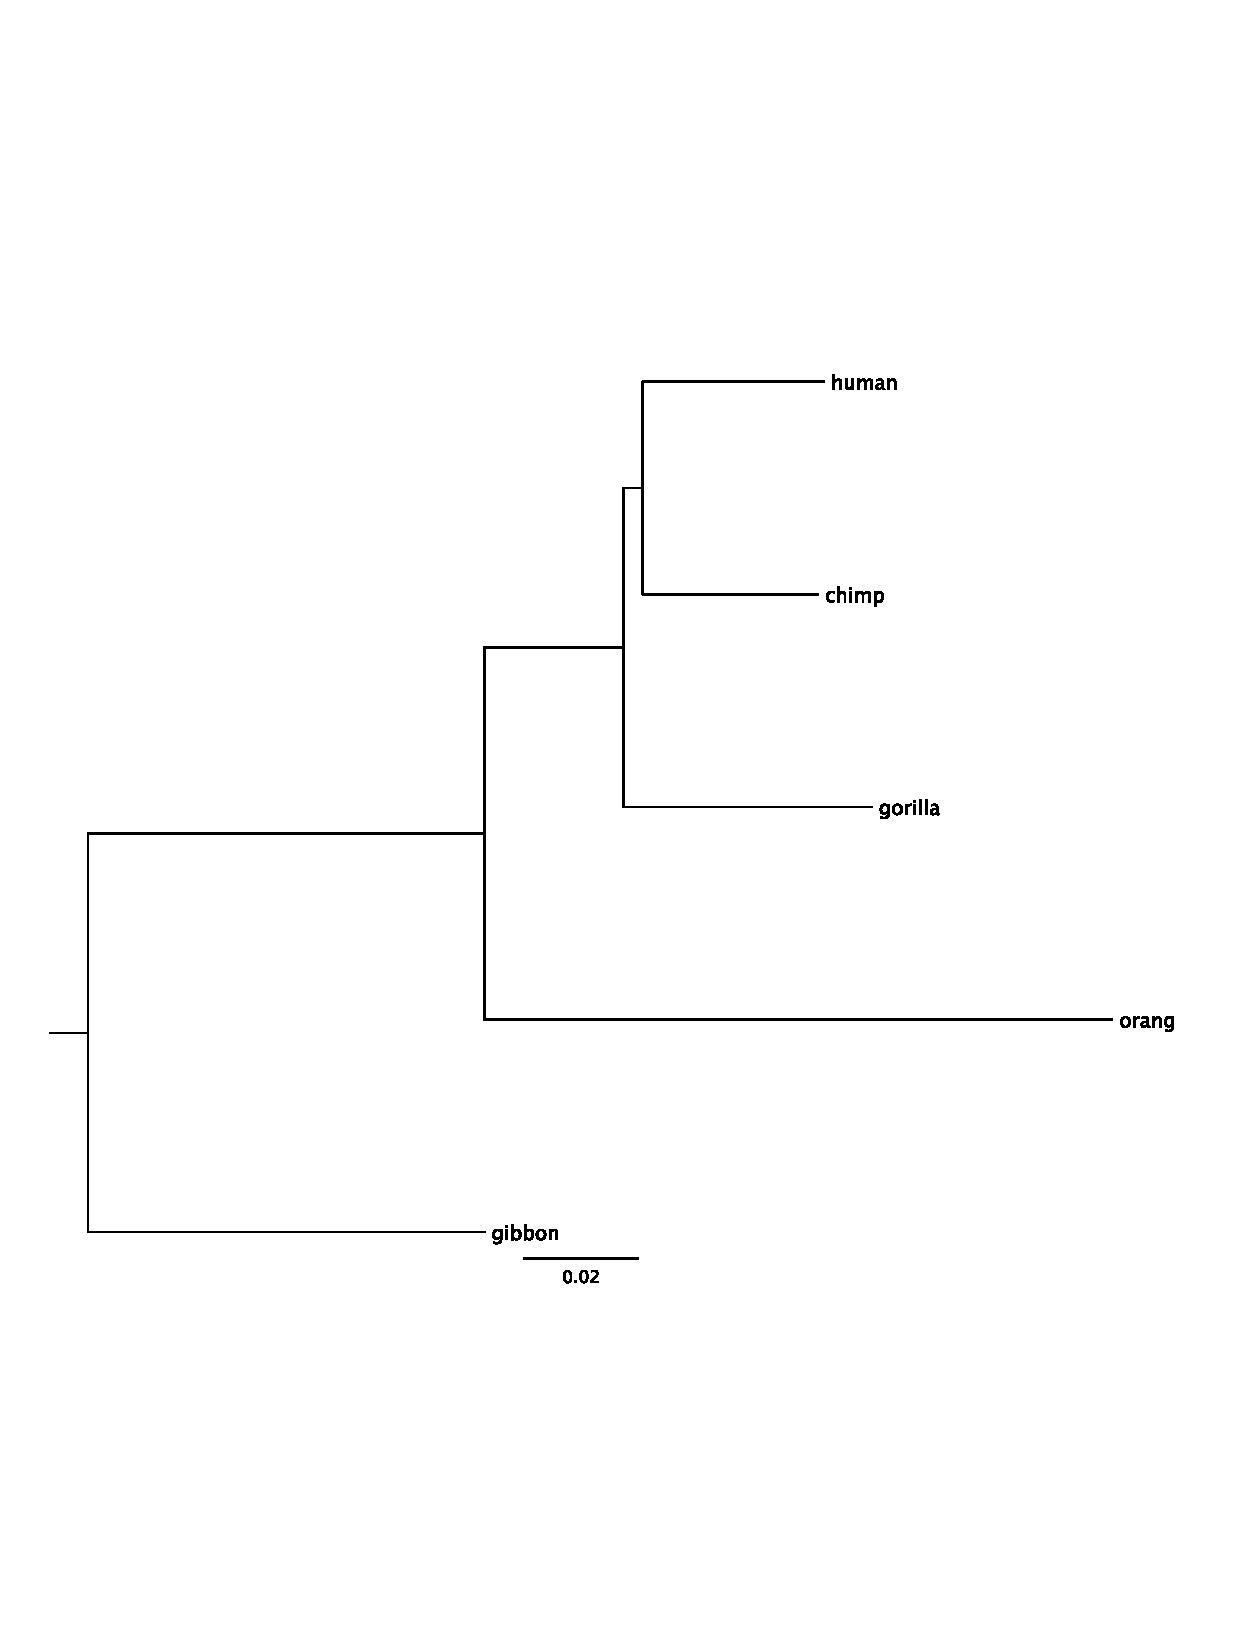
\includegraphics[scale=1.0]{../scripts/mtdna/humanChimp3000SitesTree.pdf}}}
\end{picture}

\myNewSlide
\begin{picture}(500,0)(-20,-50)
	  \put(20,-20){\small Using 3000 sites of mtDNA sequence for 5 primates}
	  \put(20,-60){\normalsize $T_1$ is ((chimp, gorilla), human)   \hskip2cm $\ln L(T_1|X) = -7363.296$}
	  \put(20,-100){\normalsize $T_2$ is ((chimp, human), gorilla)  \hskip2cm $\ln L(T_2|X) = -7361.707$}
	  \put(-10,-385){\small$\delta(T_1,T_2|X)=-3.18$}
	  \put(300,-385){\small$\mathbb{E}(\delta)$}
	  \put(50,-150){\makebox(0,-190)[l]{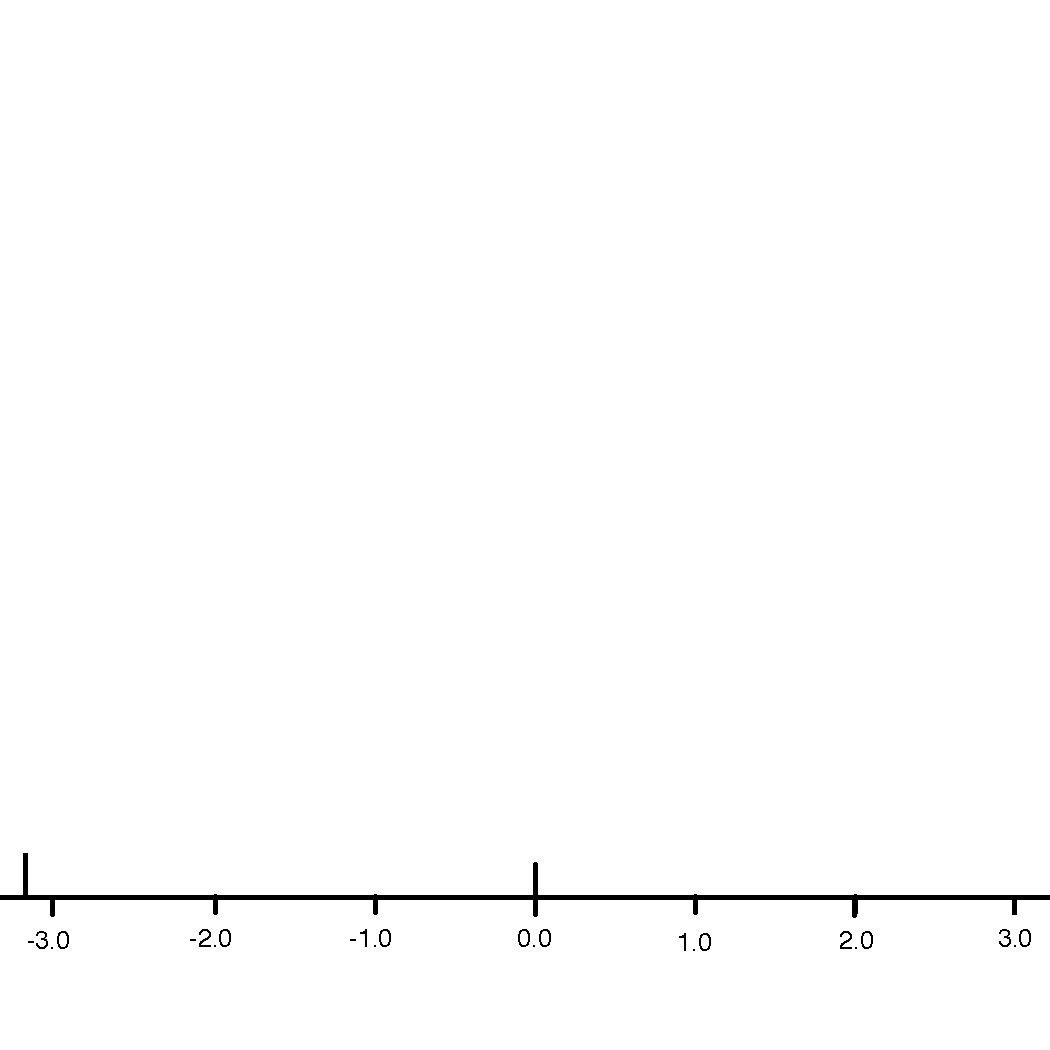
\includegraphics[scale=1.0]{../newimages/delta_axes.pdf}}}
	  \put(220,-480){$\delta(T_1,T_2|X) $}
\end{picture}




\myNewSlide

To get the $P$-value, we need to know the probability: $$\Pr\left(\big|\delta(T_1,T_2|X)\big| \geq 3.18 | H_0\mbox{ is true}\right) $$
\begin{picture}(500,0)(-20,-50)
	  \put(-10,-235){\small$\delta(T_1,T_2|X)=-3.18$}
	  \put(460,-235){\small$-\delta(T_1,T_2|X)=3.18$}
	  \put(10,-270){\huge$\leftarrow$}
	  \put(570,-270){\huge$\rightarrow$}
	  \put(300,-235){\small$\mathbb{E}(\delta)$}
	  \put(50,-0){\makebox(0,-190)[l]{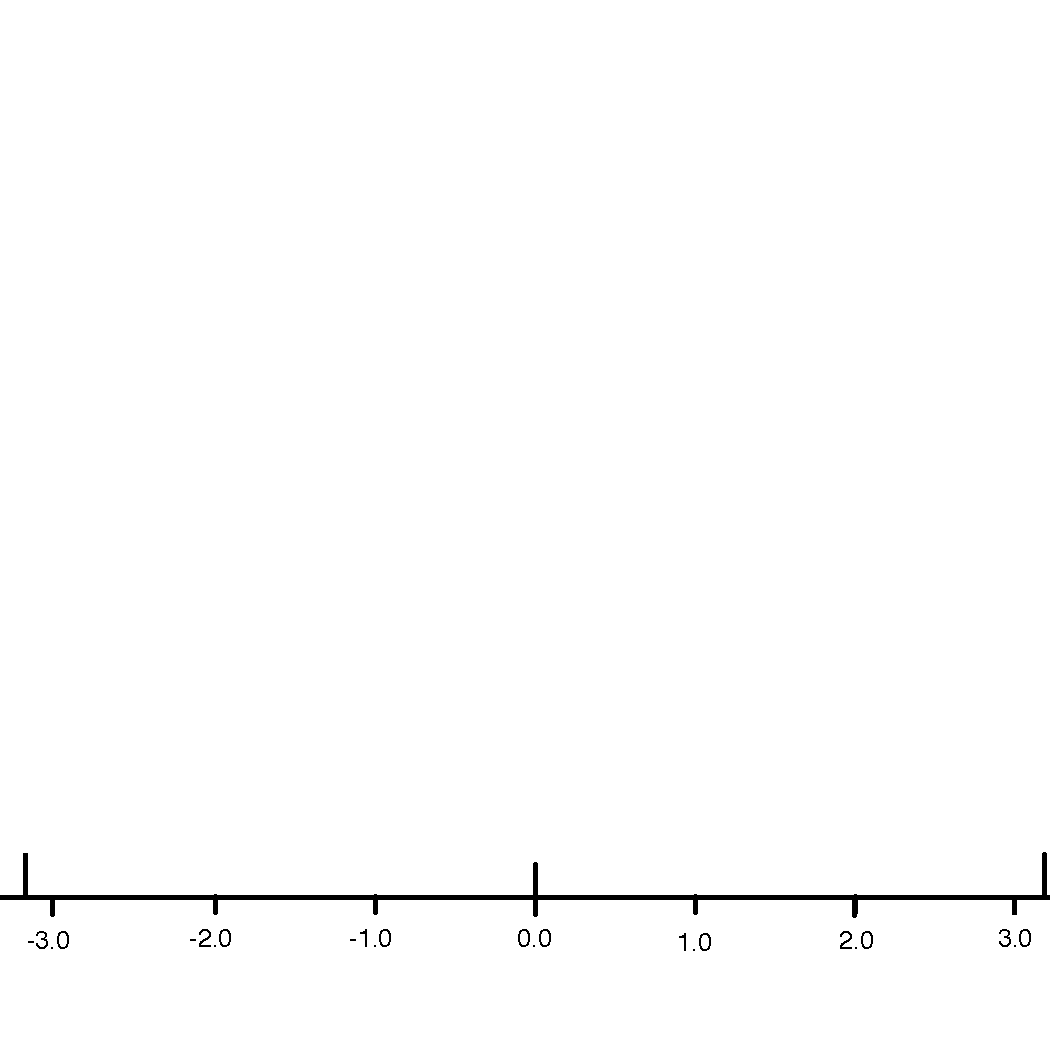
\includegraphics[scale=1.0]{../newimages/delta_axes_reflected.pdf}}}
	  \put(220,-330){$\delta(T_1,T_2|X) $}
\end{picture}

\myNewSlide
\section*{KH Test}
\begin{compactenum}
	\item Examine at the difference in $\ln L$ for each site: $\delta(T_1,T_2|X_i)$ for site $i$.
	\item Note that the total difference is simply a sum:
		$$\delta(T_1,T_2|X) = \sum_{i=1}^M\delta(T_1,T_2|X_i)$$
	\item The variance of $\delta(T_1,T_2|X)$ will be a function of the variance in ``site'' $\delta(T_1,T_2|X_i)$ values.
\end{compactenum}



\myNewSlide
\begin{picture}(500,0)(0,0)
	  \put(0,10){\large $\delta(T_1,T_2|X_i)$ for each site, $i$.}
	  \put(280,-35){\large $\vdots$}
	  \put(20,-250){\makebox(0,0)[l]{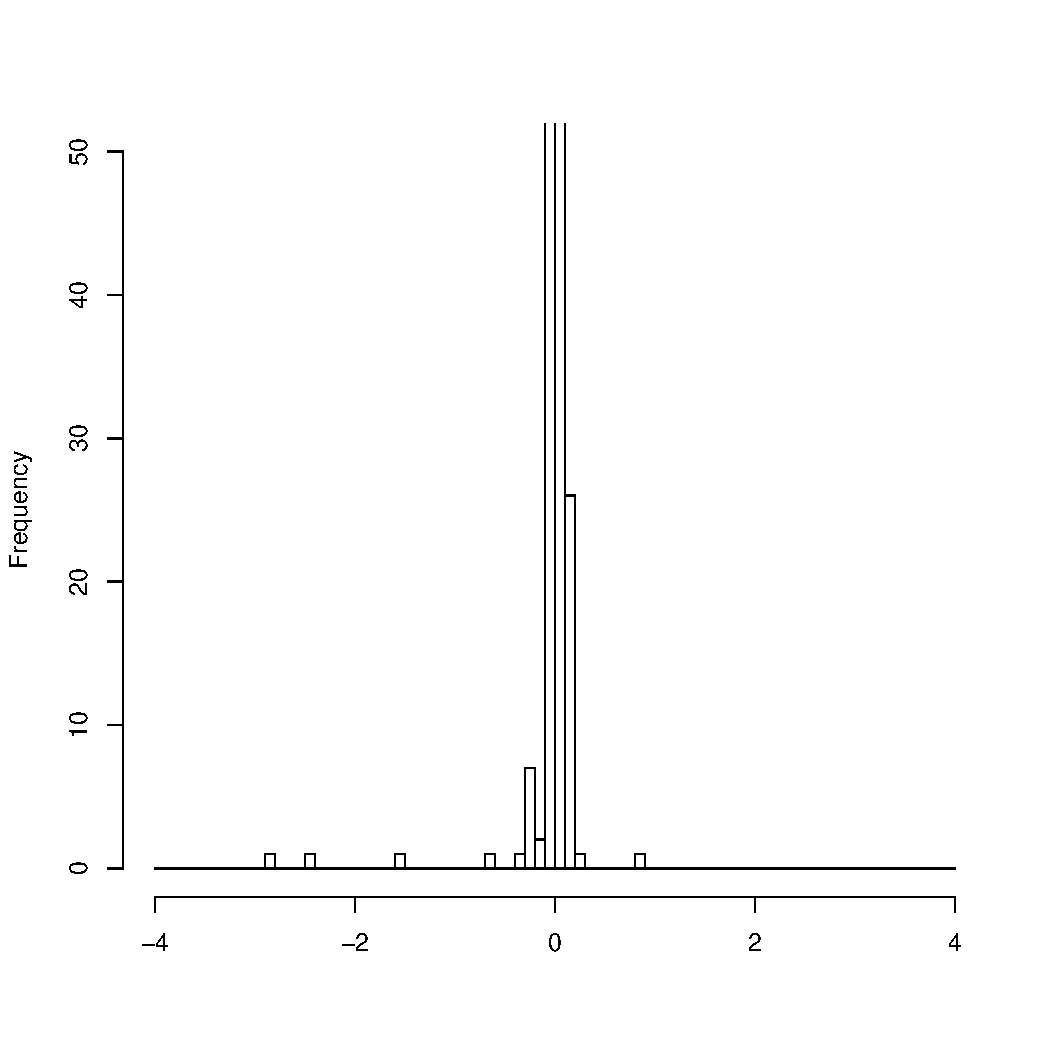
\includegraphics[scale=1.0]{../scripts/mtdna/d1-2hist.pdf}}}
	  \put(250,-490){\normalsize$\delta(T_1,T_2|x_i)$}
\end{picture}


\myNewSlide
\section*{KH Test - the variance of $\delta(T_1,T_2|X)$}
To get a sense of the variance of $\delta(T_1,T_2|X)$ we should expect because of sampling error, we could use:
\begin{compactenum}
	\item Assumptions of Normality (by appealing to the Central Limit Theorem), or
	\item Bootstrapping to generate a cloud of pseudo-replicate $\delta(T_1,T_2|X^{\ast})$ values.
\end{compactenum}

\myNewSlide
\section*{RELL bootstrap}
\large
If the MLE of the numerical parameters (including branch lengths) do not change much when we bootstrap we can simply resample the site $\ln L$ values and sum them.

This is called the RELL bootstrap \citep[][and Felsenstein]{KishinoMH1990}. It is not a ``safe'' replacement for normal bootstrapping \citep[especially on large trees;][]{StamatakisHR2008} when you want to estimate clade support.

But it should be good enough for helping us learn about the standard error of the $\ln L$.

And it is really fast.

\myNewSlide
\begin{picture}(500,0)(0,0)
	  \put(0,-10){\large $\delta$ for many (RELL) bootstrapped replicates of the data}
	  \put(20,-250){\makebox(0,0)[l]{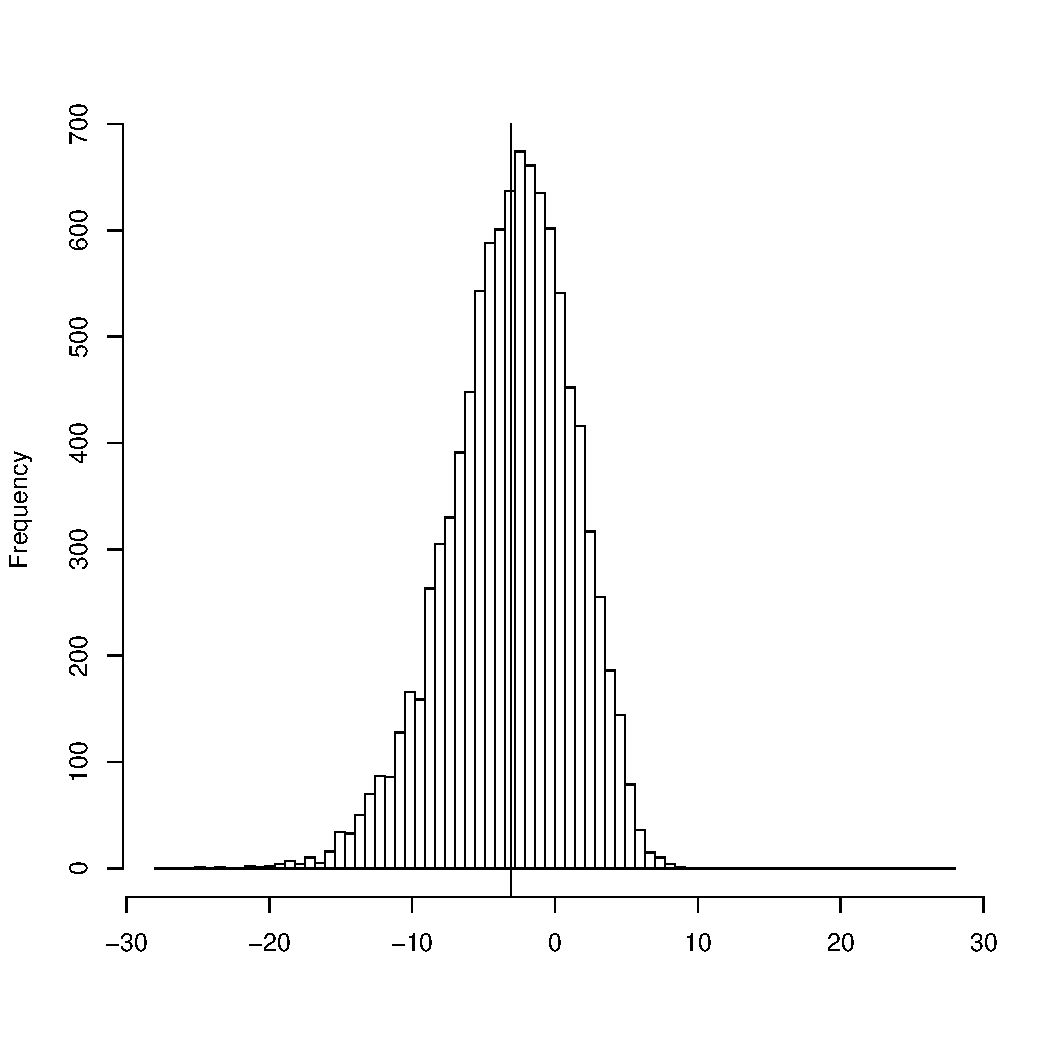
\includegraphics[scale=1.0]{../scripts/mtdna/uncentered1-2hist.pdf}}}
	  \put(250,-490){\normalsize$\delta(T_1,T_2|X^{\ast})$}
\end{picture}

\myNewSlide
\section*{KH Test - `centering'}
$H_0$ gives us the expected value: $$\mathbb{E}_{H_0}\left[\delta(T_1,T_2|X)\right] = 0$$
Bootstrapping gives us a reasonable guess of the variance under $H_0$

By substracting the mean of the bootstrapped $\delta(T_1,T_2|X^{\ast})$ values, we can create a null distribution.

For each of the $j$ bootstrap replicates, we treat $$\delta(T_1,T_2|X^{\ast j}) - \bar\delta(T_1,T_2|X^{\ast})$$  as draws from the null distribution.

\myNewSlide
\begin{picture}(500,0)(0,0)
	  \put(0,10){\large $\delta(T_1,T_2|X^{(j)})-\bar\delta(T_1,T_2|X^{\ast})$}
	  \put(0,-25){for many (RELL) bootstrapped replicates of the data}
	  \put(20,-250){\makebox(0,0)[l]{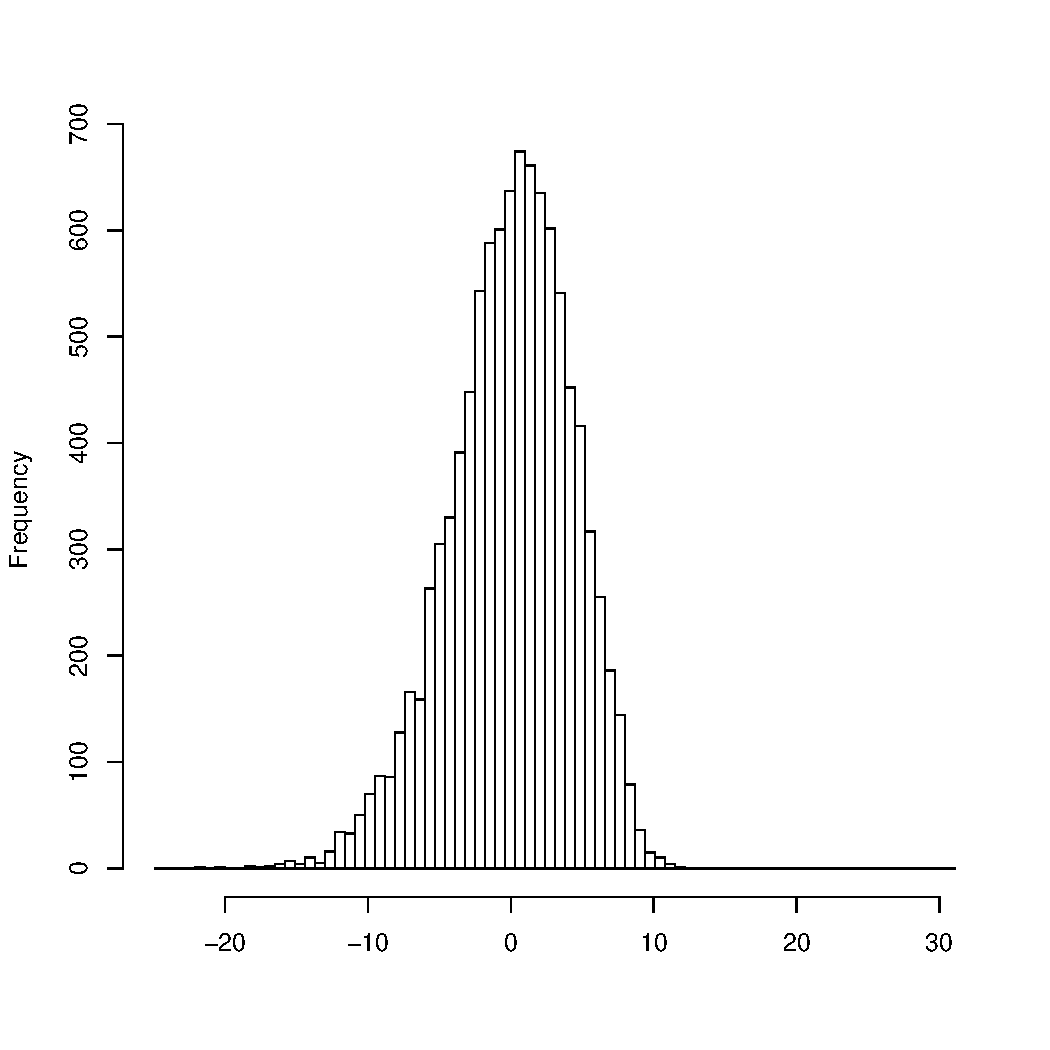
\includegraphics[scale=1.0]{../scripts/mtdna/centered1-2hist.pdf}}}
	  \put(150,-490){\normalsize$\delta(T_1,T_2|X^{(j)})-\bar\delta(T_1,T_2|X^{\ast})$}
\end{picture}

\myNewSlide
\begin{picture}(500,0)(0,0)
	  \put(0,10){\large $\delta(T_1,T_2|X^{(j)})-\bar\delta(T_1,T_2|X^{\ast})$}
	  \put(0,-25){for many (RELL) bootstrapped replicates of the data}
	  \put(20,-250){\makebox(0,0)[l]{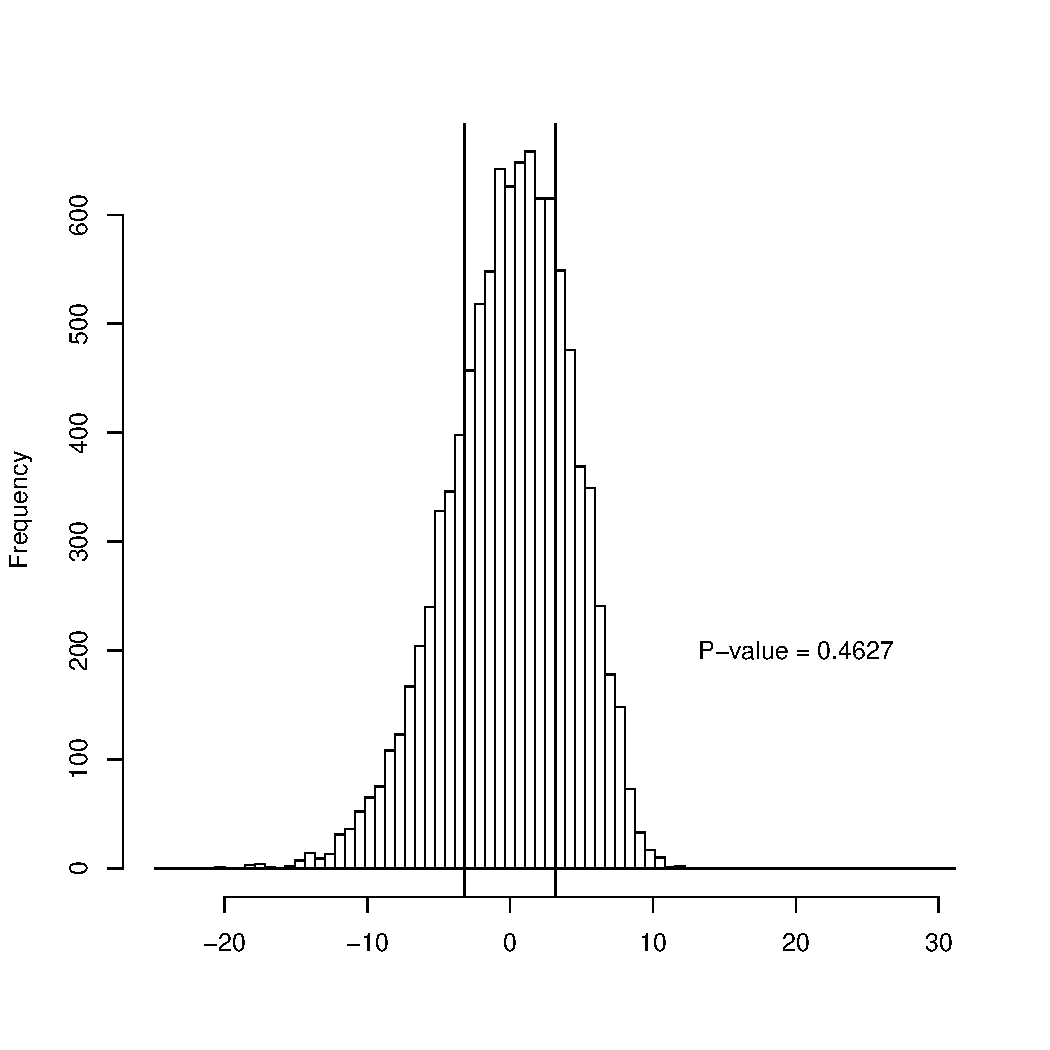
\includegraphics[scale=1.0]{../scripts/mtdna/centered1-2hist-p.pdf}}}
	  \put(250,-490){\normalsize$\delta(T_1,T_2|X^{\ast})-\bar\delta(T_1,T_2|X^{\ast})$}
\end{picture}


\myNewSlide
\section*{What if start out with only one hypothesized tree, and we want to compare it to the ML tree?}
The KH Test is {\bf NOT} appropriate in this context \citep[see][for discussion of this point]{GoldmanAR2000}
	
{\bf Multiple Comparisons}: lots of trees increases the variance of $\delta(\hat{T},T_1|X)$\\

{\bf Selection bias}: Picking the ML tree to serve as one of the hypotheses invalidates the centering procedure of the KH test.

\myNewSlide
\section*{Using the ML tree in your test introduces selection bias}
Even when the $H_0$ is true, we do not expect $2\left[\ln L(\hat{T}) - \ln L(T_1)\right]= 0$

Imagine a competition in which a large number of equally skilled people compete, and you compare the score of one competitor against the highest scorer.

\myNewSlide
\begin{picture}(500,0)(0,0)
	  \put(-10,15){Experiment: 70 people each flip a fair coin 100 times and}
	  \put(0,-20){count \# heads.  Test statistic:}
	  \put(100,-55){$h_1 - h_2$}
	  \put(400,-55){$\max(h) - h_1$}
	  \put(-30,-250){\makebox(0,0)[l]{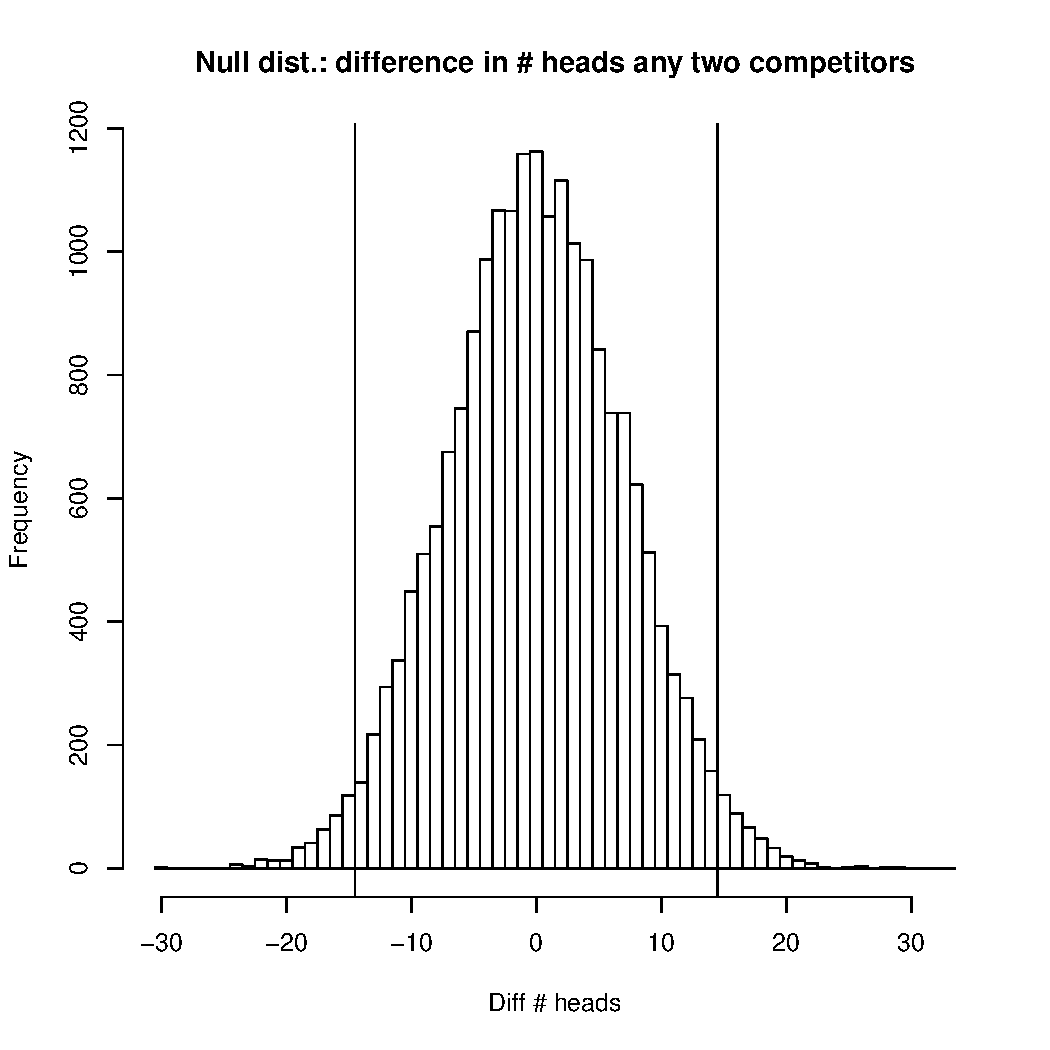
\includegraphics[scale=.75]{../scripts/cfc_diff_a_priori.pdf}}}
	  \put(320,-250){\makebox(0,0)[l]{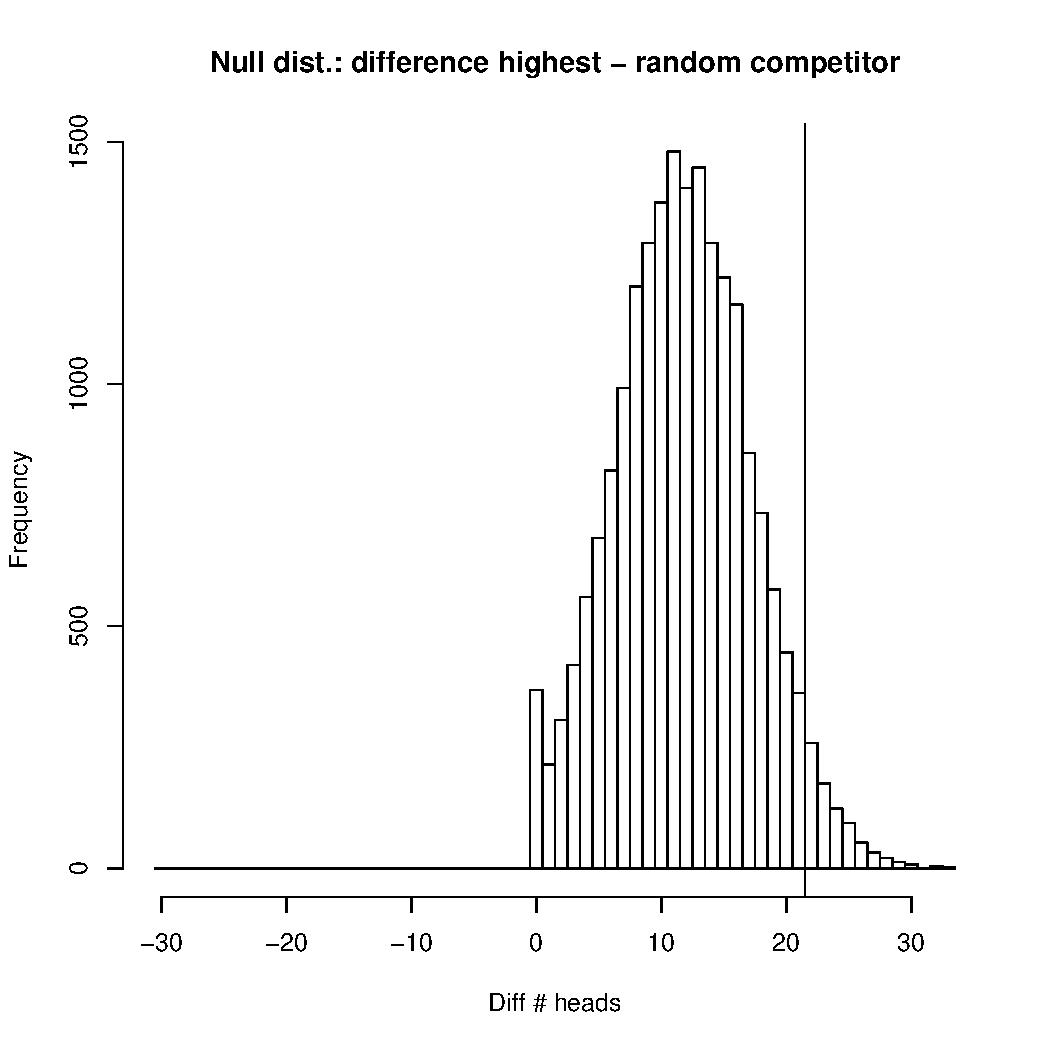
\includegraphics[scale=.75]{../scripts/cfc_diff_best_v_one.pdf}}}
\end{picture}


\myNewSlide 
\section*{Shimodaira and Hasegawa proposed the SH test which deals the ``selection bias'' introduced by using the ML tree in your test}
You have to specify of a set of candidate trees - inclusion in this set {\bf must not} depend on the dataset to be analyzed.

The null hypothesis is that all members of the candidate set have the same expected score.

\myNewSlide
{\bf SH Test details}
\normalsize
\begin{compactitem}
	\item For each tree $T_i$ in the candidate set calculate $\delta(\hat{T}, T_i|X)$
	\item Bootstrap to generate ${\ln L}(T_i|X^{(j)})$
	\item For each tree $T_i$, use $\bar{\ln L}(T_i|X^{\ast})$ to center the bootstrapped collection of log-likelihoods:
		$$c_i^{(j)} = {\ln L}(T_i|X^{(j)})-\bar{\ln L}(T_i|X^{\ast})$$
	\item For each replicate pick the highest value from the centered distributions (this mimics the selection bias): $$m^{(j)} = \max\left[c_i^{(j)}\right] \mbox{ over all } j$$
	\item The for each tree and replicate, you get a sample from the null $\delta_i^{(j)} = m^{(j)} - c_i^{(j)}$
	\item $P$-value for tree $T_i$ can be approximated by seeing where in the distribution of $\delta_i^{(j)}$ values it lies (the $P$-value is the proportion of sampled $\delta_i^{(j)} \geq \delta_i$
\end{compactitem}

\myNewSlide
\section*{SH test candidate set selection}
\large
\begin{compactitem}
	\item The candidate set should be all trees that you would have seriously entertained before seeing the data. 
	\item Using all trees is safe (though weakens the test, and is computationally demanding).
	\item Unfortunately, only considering a subset of trees for computational convenience can invalidate the test.
	\item If a tree has low $\ln L$ and low variance of site-log-likelihoods then it can probably be safely removed without affecting the $P$-values of other trees\footnote{Because such a tree would be unlikely to ever be the tree that is the determines the maximum diplacement from the centered value, $m^{(j)}$.}
\end{compactitem}
The test makes worst-case assumptions, so the SH test {\bf is too conservative}.

\myNewSlide
\large
\begin{picture}(500,0)(0,0)
	  \put(-200,-190){\makebox(0,0)[l]{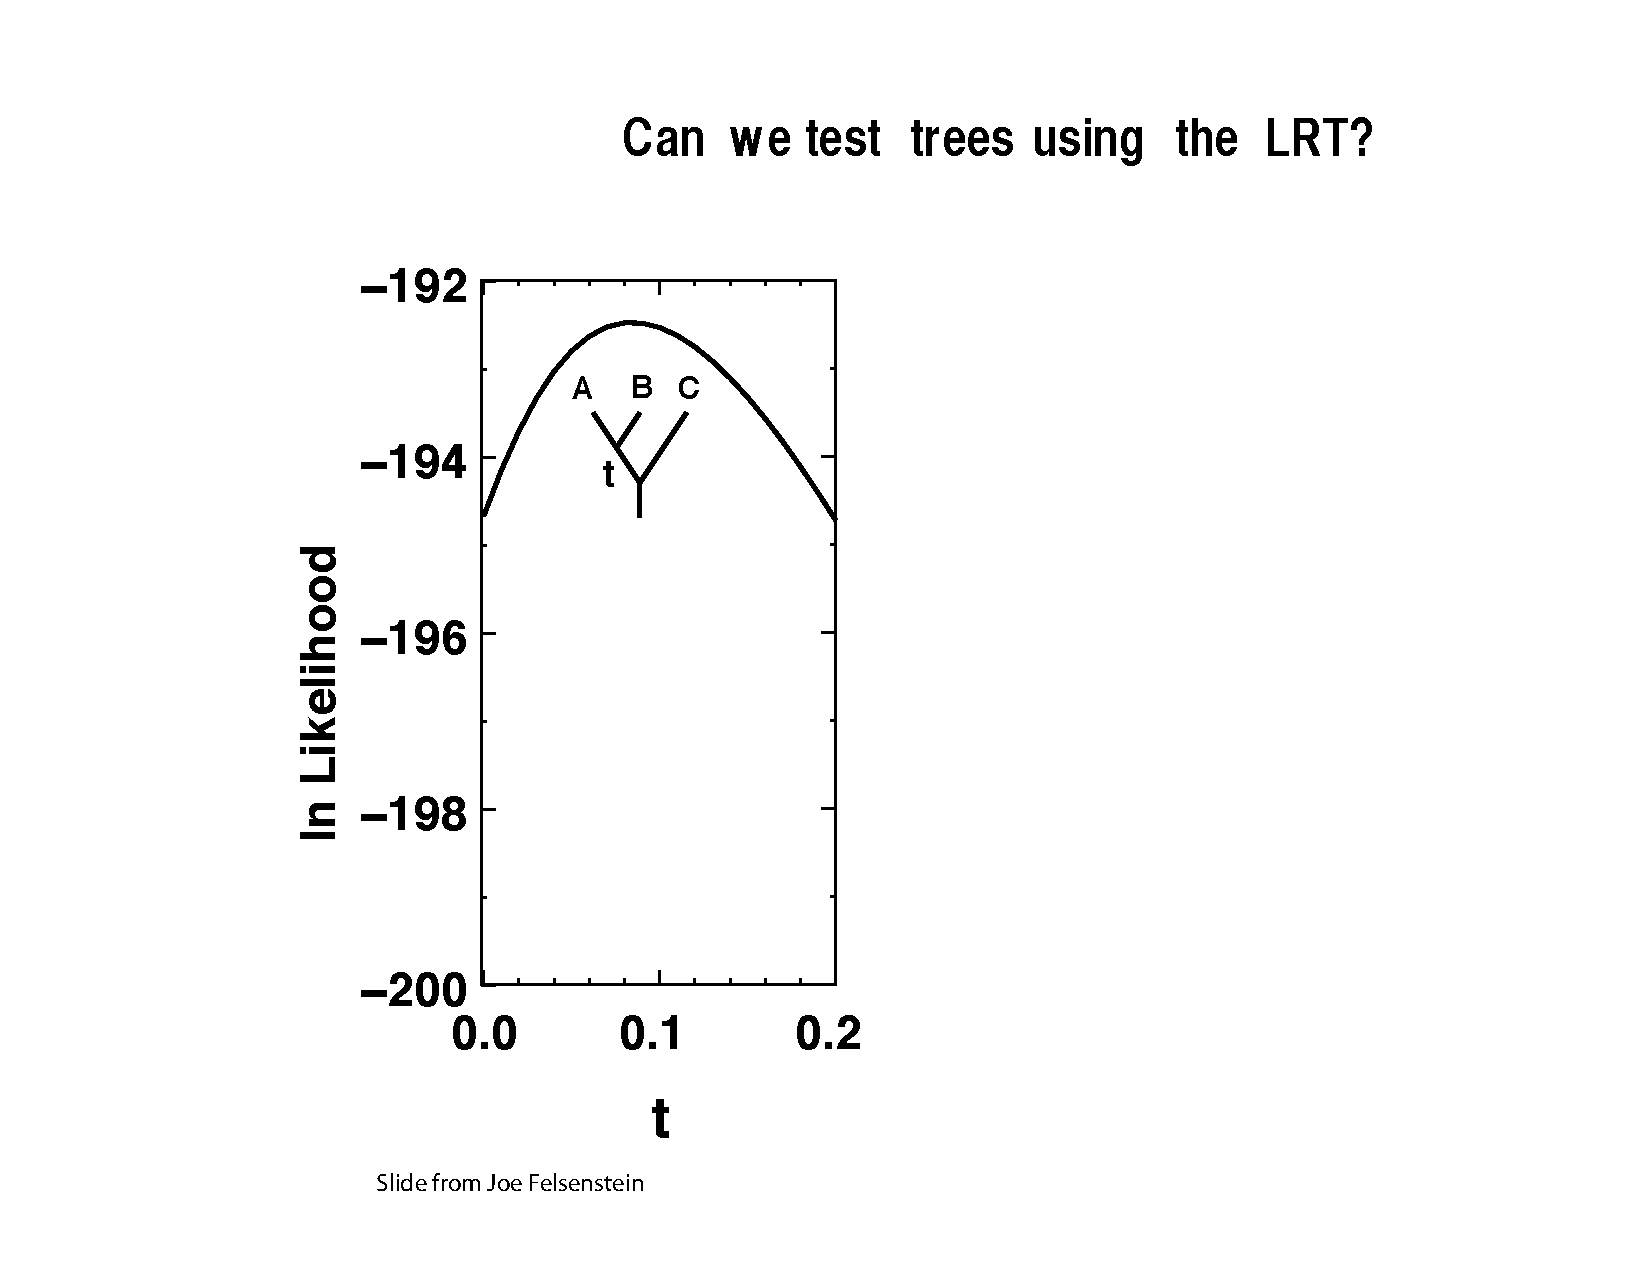
\includegraphics[scale=1.0]{../newimages/JoeFelsTreeLRT1.pdf}}}
	  \put(250,-100){1. Should we calculate the LRT as:}
	  \put(230,-140){$\delta_i = 2\left[\ln L(t=\hat{t},T_i|X) - \ln L(t=0,T_i|X)\right]$}
	  \put(250,-250){2. And can we use the $\chi_1^2$ distribution to}
	  \put(250,-290){get the critical value for $\delta$?}
\end{picture}

\myNewSlide
\begin{picture}(500,0)(0,0)
	  \put(-200,-190){\makebox(0,0)[l]{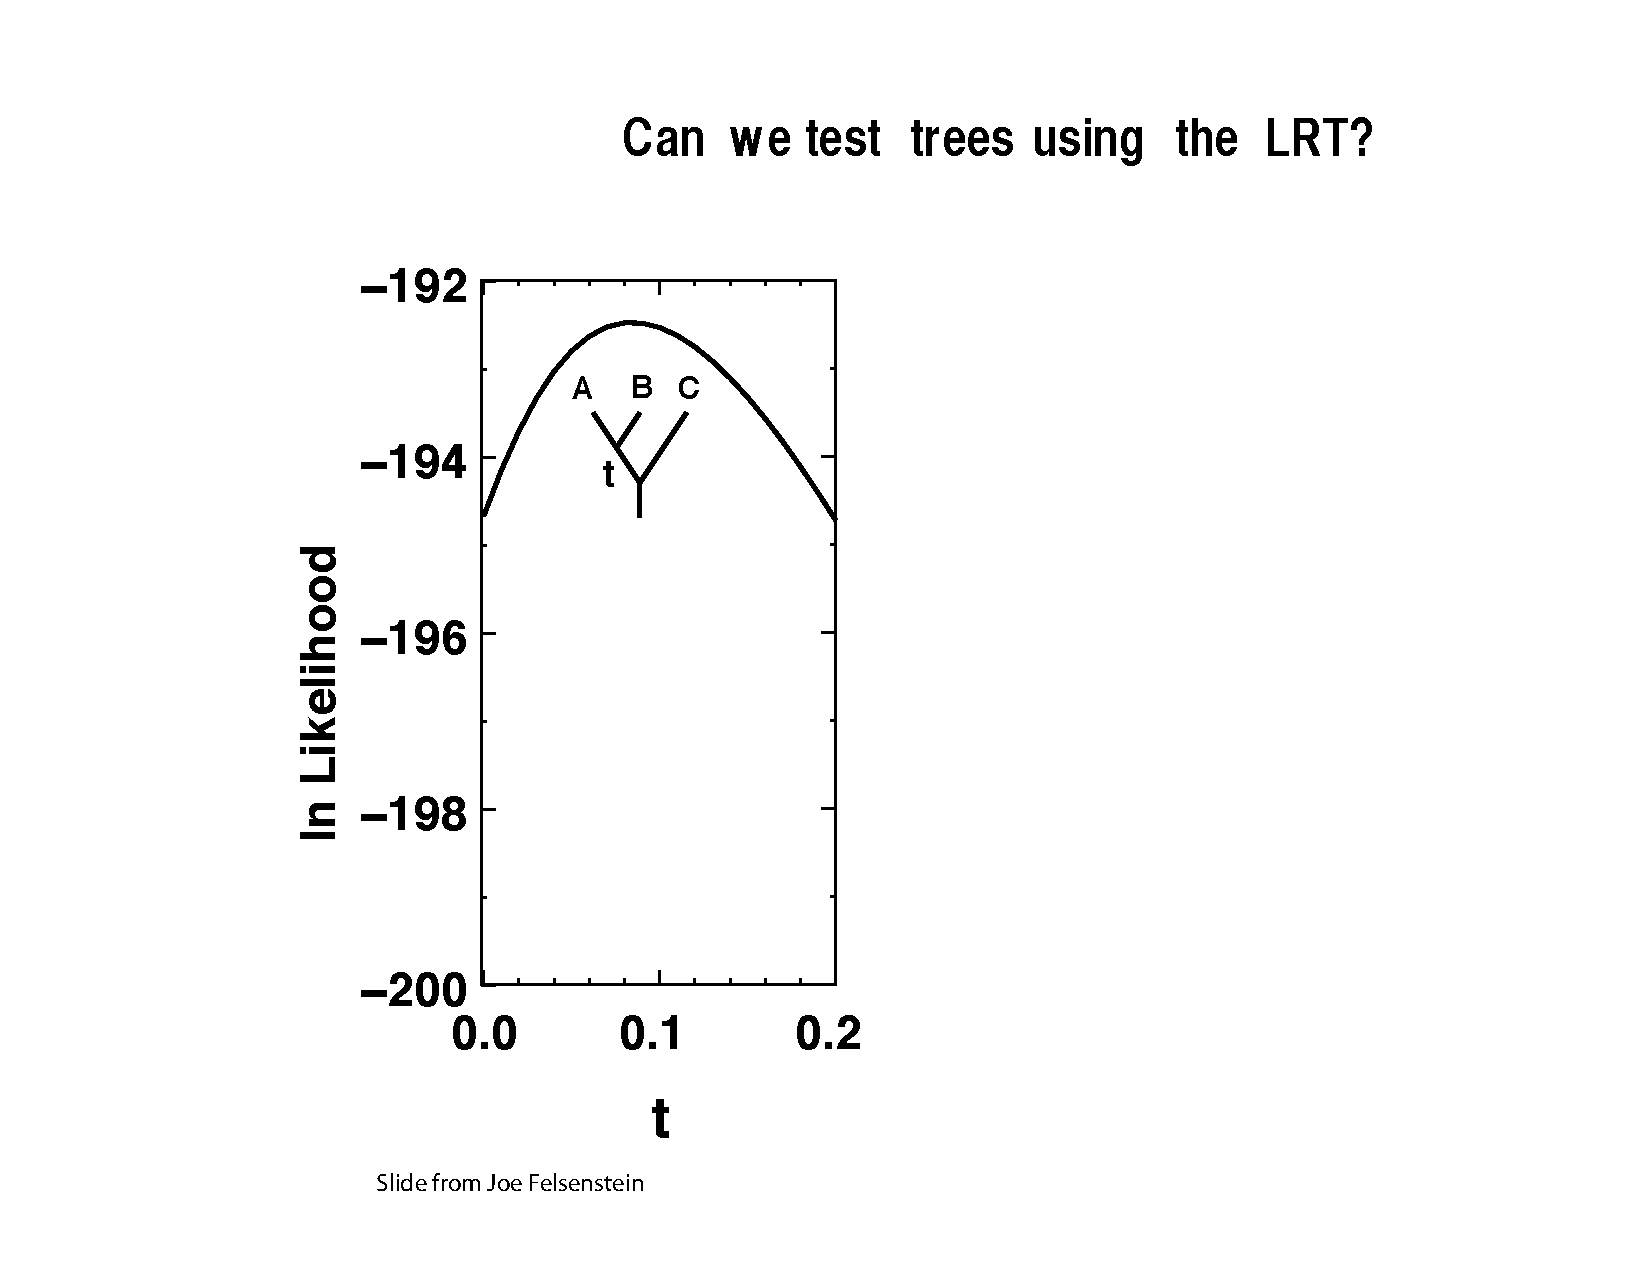
\includegraphics[scale=1.0]{../newimages/JoeFelsTreeLRT1.pdf}}}
	  \put(250,-100){1. Should we calculate the LRT as:}
	  \put(230,-140){$\delta_i = 2\left[\ln L(t=\hat{t},T_i|X) - \ln L(t=0,T_i|X)\right]$}
	  \put(250,-180){{\bf \color{red}No. $t=0$ might not yield the best}}
	  \put(260,-220){\bf\color{red} alternative $\ln L$}
	  \put(250,-290){2. And can we use the $\chi_1^2$ distribution to}
	  \put(250,-330){get the critical value for $\delta$ ?}
	  \put(250,-370){{\bf \color{red}No. Constraining parameters}}
	  \put(260,-410){{\bf \color{red}at boundaries leads to a mixture}}
	  \put(260,-450){{\bf \color{red}such as: $\frac{1}{2}\chi_0^2 + \frac{1}{2}\chi_1^2$}}
	  \put(260,-490){\small See \citet{OtaWHSK2000}.}
\end{picture}

\myNewSlide
\begin{picture}(500,0)(0,0)
	  \put(-200,-190){\makebox(0,0)[l]{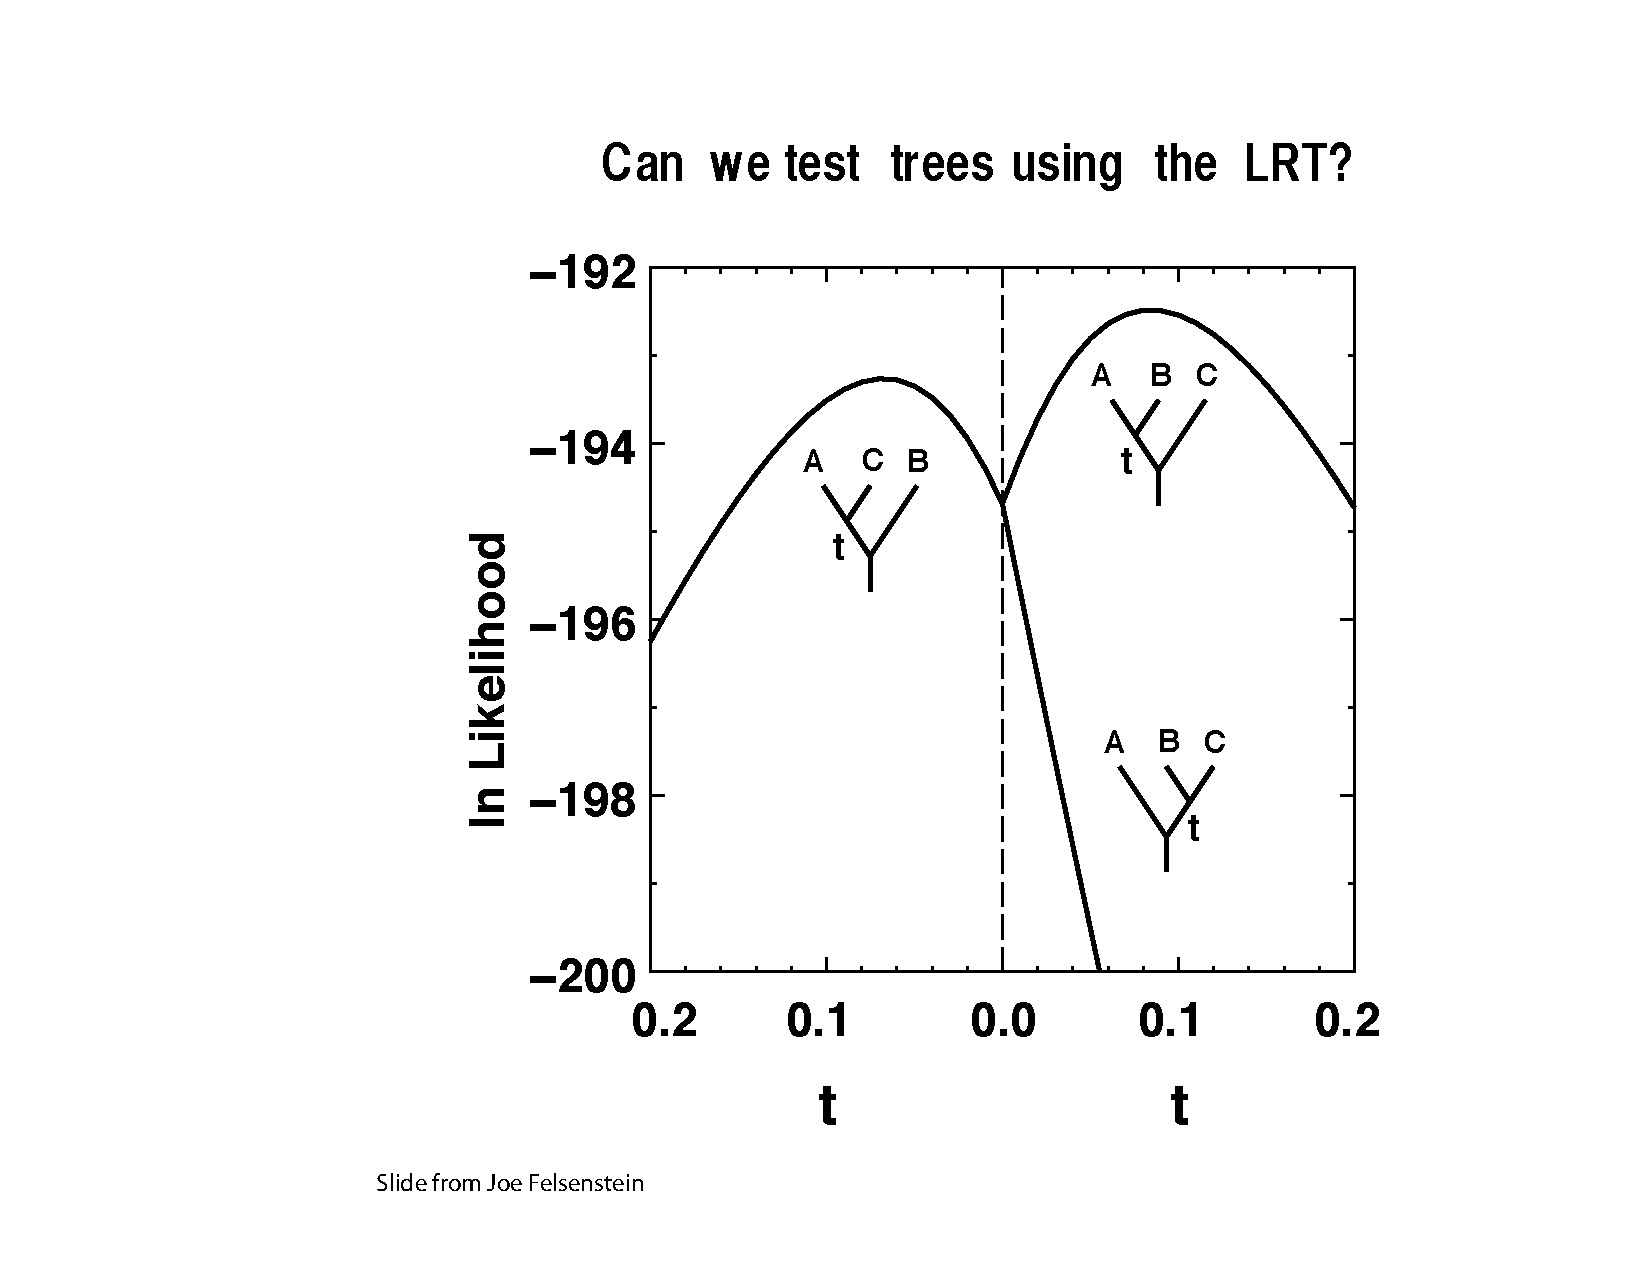
\includegraphics[scale=1.0]{../newimages/JoeFelsTreeLRT2.pdf}}}
\end{picture}

\myNewSlide
\section*{Parametric bootstrapping}
Generate the null distribution of $\delta_i$ by:
\begin{compactitem}
	\item finding the best tree and model pair that are consistent with the $H_0$,
	\item Simulating a large number $B$ of data sets, $X^{(1)}, X^{(2)},\ldots,X^{(B)}$ according to the parameters of that model,
	\item Calculating $\delta^{(j)} = 2\left[\ln L (\hat{T}; X^{(j)}) - \ln L (\hat{T}_{0}; X^{(j)})\right]$ where $\hat{T}_{0}$ is the tree estimated when you enforce a constraint such that all of the trees are compatible with the null.
\end{compactitem}

\myNewSlide
\section*{Parametric bootstrapping}
Intuitive and powerful, but not robust to model violation \citep{Buckley2002}.

In the SOWH test, the null tree is specified {\em a priori}.

\myNewSlide
\includepdf[pages={1}]{/Users/mholder/Documents/ku_teaching/BIOL-848-2010/images/gtr_i_g_sim_hist_data.pdf} 


\myNewSlide
\includepdf[pages={1}]{/Users/mholder/Documents/ku_teaching/BIOL-848-2010/images/jc_sim_hist_data.pdf} 

\myNewSlide
\section*{aLRT of \citet{AnisimovaG2006}}
\begin{compactitem}
	\item For a {\bf branch} $j$, calculate $\delta_{j}^{\dag}$ as twice the difference in $\ln L$ between the optimal tree (which has the branch) and the best NNI neighbor that lacks the branch.
	\item This is very fast, and can be done in PhyML.
	\item The argue that the null distribution for each LRT around the polytomy follows a $\frac{1}{2}\chi_0^2 + \frac{1}{2}\chi_1^2$ distribution
	\item The introduce Bonferroni-correction appropriate for correcting for the selection of the best of the three resolutions.
	\item They find aLRT to be accurate and powerful in simulations, but \citet{AnisimovaGDDG2011} report that it rejects too often and is sensitive to model violation.
\end{compactitem}

\myNewSlide
\begin{picture}(500,0)(0,0)
	  \put(-130,-450){\makebox(0,0)[l]{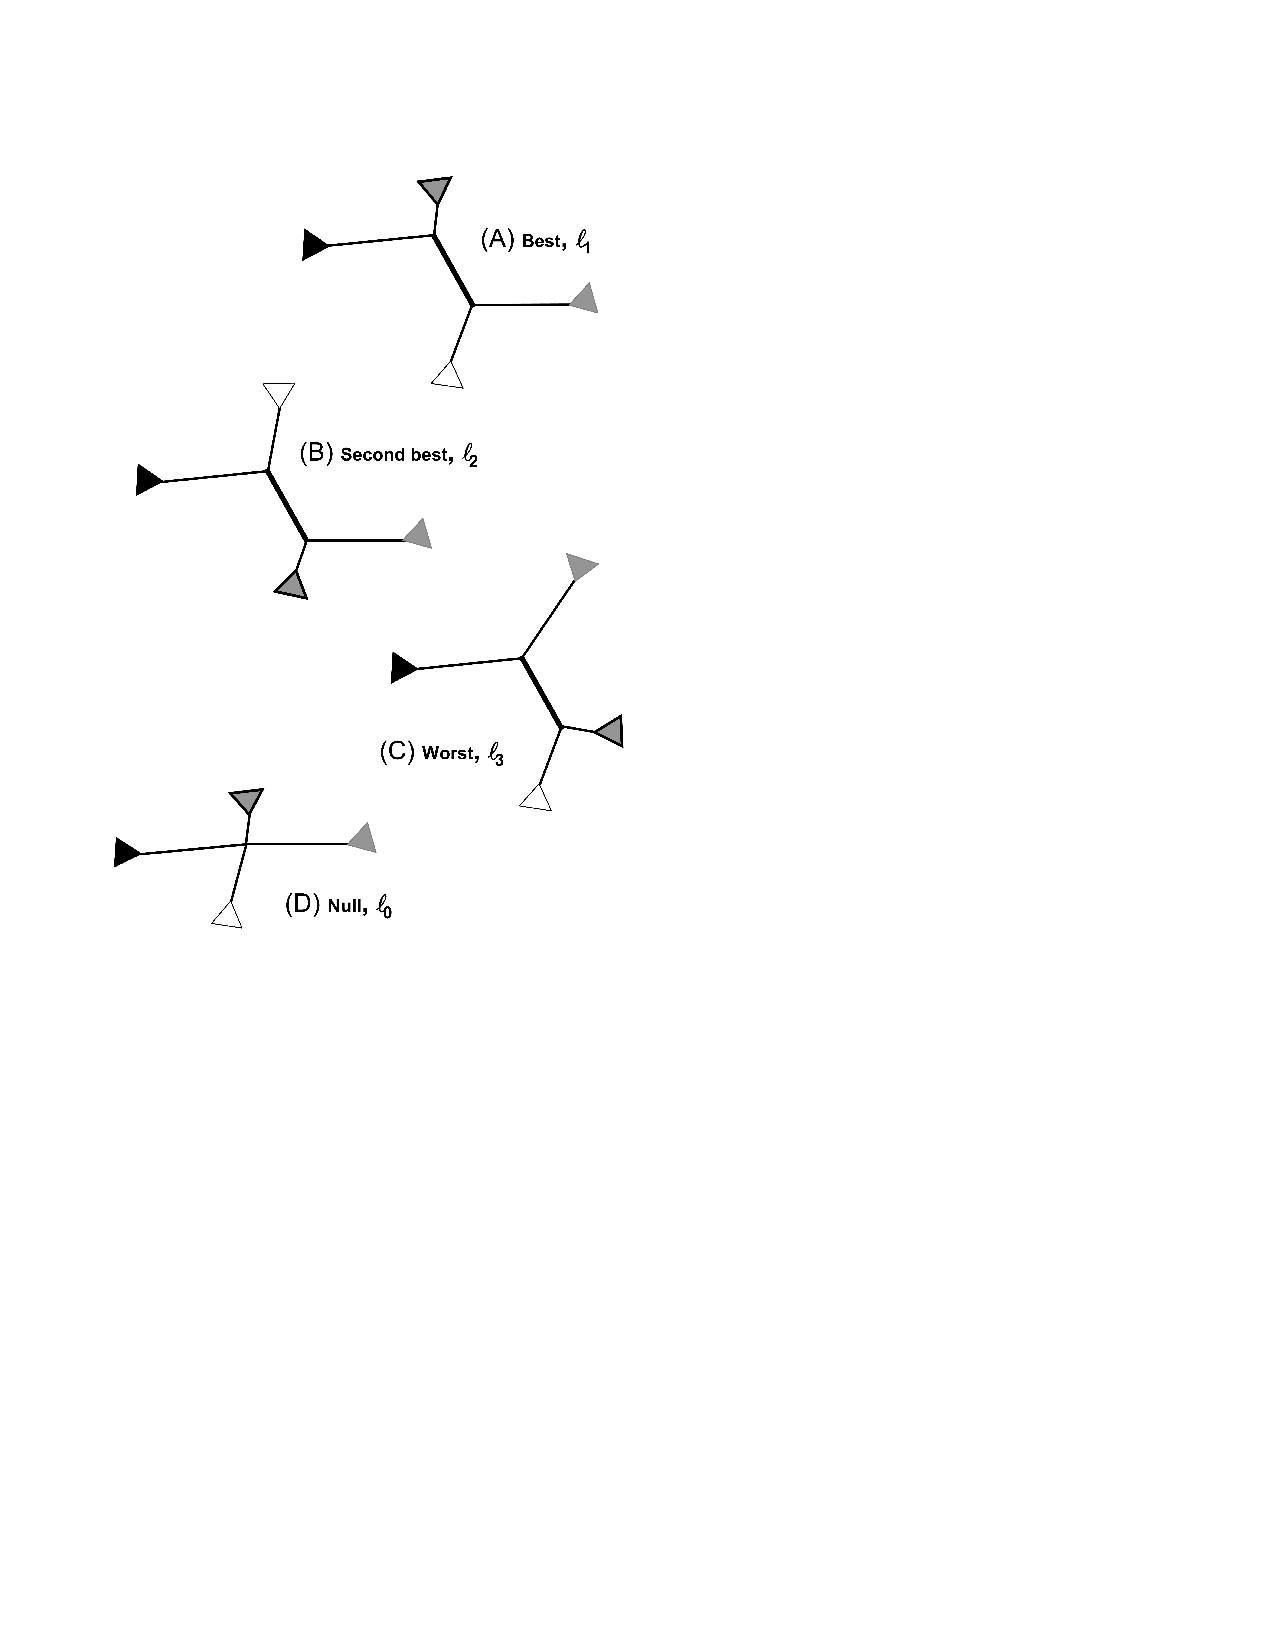
\includegraphics[scale=1.5]{../newimages/AnisimovaG2006Fig1.pdf}}}
	  \put(330,-200){aLRT = $2\left[\ln L(T_1|X) - \ln L(T_2|X)\right]$}
	  \put(400,-400){\small Image from \citet{AnisimovaG2006}}
\end{picture}

\myNewSlide
\section*{aBayes \citet{AnisimovaGDDG2011} }


$$\mbox{aBayes}(T_1|X) = \frac{\Pr(X|T_1}{\Pr(X|T_1) + \Pr(X|T_2) + \Pr(X|T_3)}$$

Simulation studies of \citet{AnisimovaGDDG2011} show it to have the best power of the methods that do not have inflated probability of falsely rejecting the null.

It is sensitive to model violation.

This is similar to ``likelihood-mapping'' of \citet{StrimmerVH1997}




\myNewSlide
\large
Bootstrap proportions have been characterized as providing:
\begin{compactitem}
	\item a measure of repeatability,
	\item an estimate of the probability that the tree is correct (and bootstrapping has been criticized as being too conservative in this context),
	\item the P-value for a tree or clade
\end{compactitem}





\myNewSlide
\section*{Bootstrap Proportion $\neq$ Posterior Probability}
Several studies have compared the non-parametric bootstrap proportion of clade from an ML analysis of a data set to the posterior probabilities when the same data is analyzed under the same model \citep{SuzukiGN2002,WilcoxZHH2002,AlfaroZL2003,CummingsHMRRW2003,DouadyDBDD2003}.\par

Note: {\em \bf Not} all of these have implied that the measures {\em\bf should} be the same, but some authors have, usually citing \citet{EfronHH1996}.

\myNewSlide
\section*{Bootstrap Proportion $\neq$ Posterior Probability in general}
\begin{picture}(-0,0)(-0,0)
	\put(40,-50){\makebox(30,-150)[l]{\includegraphics[scale=2]{/Users/mholder/Documents/ku_teaching/BIOL-848-2010/images/WilcoxZHH-figure.pdf}}}
	\put(40,-330){from \citet{WilcoxZHH2002}}
\end{picture}


\myNewSlide
\section*{\citet{Newton1996} showed that, when you look at the median, the BP may not be biased downward}
\begin{picture}(-0,0)(-0,0)
	\put(40,-50){\makebox(30,-150)[l]{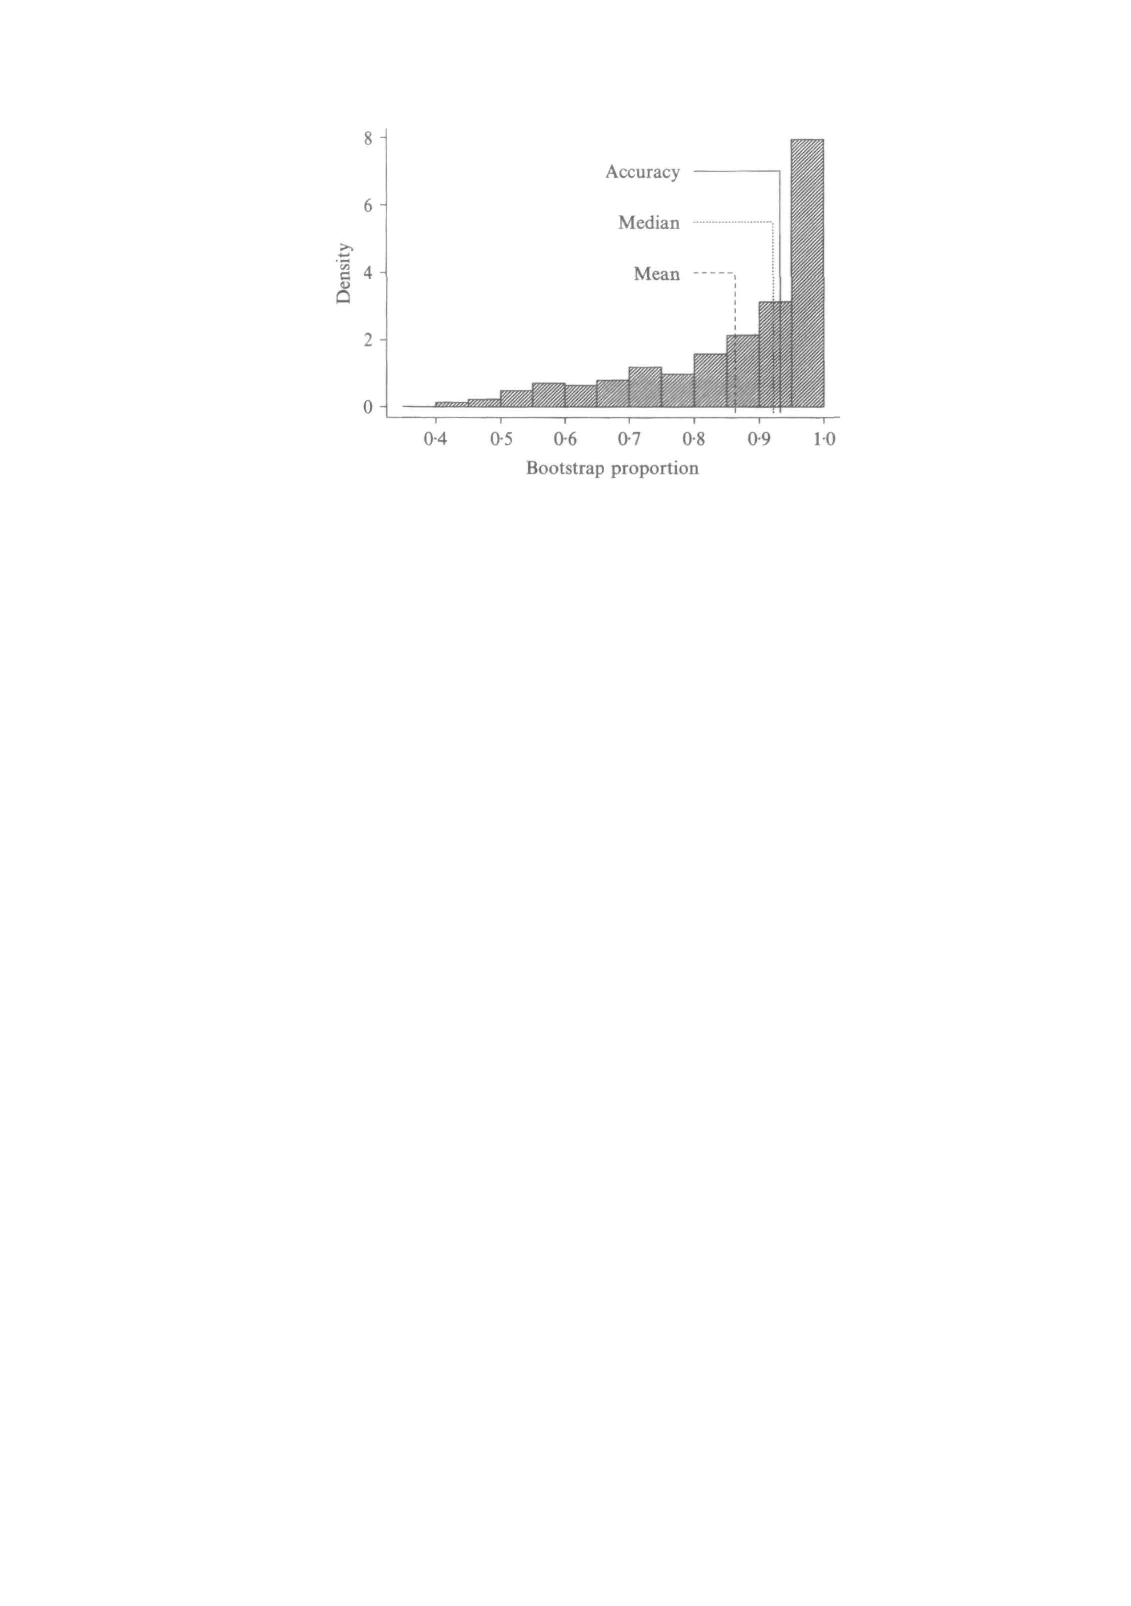
\includegraphics[scale=2]{../newimages/Newton1996Fig4.pdf}}}
	\put(40,-330){Figure 4 from \citet{Newton1996}}
\end{picture}

\myNewSlide
\section*{What did \citet{EfronHH1996} say?}
\normalsize
We can use a Bayesian model to show that $\tilde{\alpha}$ is a reasonable 
assessment of the probability that $\mathscr{R}_1$ contains $ \mu$.
Suppose we believe \textit{a priori} that $\mu$ could lie anywhere in the plane with 
equal probability. 
Then having observed $\hat{\mu}$, the \textit{a posteriori} 
distribution of  $\mu$ given  $\hat{\mu}$ is $N_2( \hat{\mu},I)$ exactly the same as the 
bootstrap distribution of $\hat{\mu}^{\ast}$. 
In other words, $\tilde{\alpha}$ is the  \textit{a posteriori}
probability of the event $\mu \in \mathscr{R}_1$, if we begin with an ``uninformative'' prior density for $\mu$.
\begin{picture}(-0,0)(-0,0)
	\put(0,-120){\makebox(30,-150)[l]{\includegraphics[scale=4]{/Users/mholder/Documents/ku_teaching/BIOL-848-2010/images/EfronHH-straight-fig.pdf}}}
\end{picture}

\myNewSlide
\section*{\citet{EfronHH1996} view of tree space}
\begin{picture}(-0,0)(-0,0)
	\put(-10,-90){\makebox(30,-150)[l]{\includegraphics[scale=3]{/Users/mholder/Documents/ku_teaching/BIOL-848-2010/images/EfronHH-treespace-fig.pdf}}}
\end{picture}

\myNewSlide
\section*{What did \citet{EfronHH1996} say (and mean)?}
\begin{itemize}
	\item the ``uninformative'' prior density is a uniform prior over all of pattern frequency space
	\item this is {\em not} equivalent to a prior that would be expected to yield a phylogeny (it is actually identical to the prior you would get if you assumed that all pairwise distances between taxa were $\infty$),
	\item  \citet{EfronHH1996}  were {\em not} predicting that the bootstrap proportions should be identical to those from a Bayesian phylogenetic analysis with real phylogenetic priors.
	\item  \cite{SvennbladEOB2006} have a nice paper on this subject.
\end{itemize}


\myNewSlide
\section*{\citet{Newton1996} provides an intuition for why the mean BP may be lower than repeatability}
\begin{picture}(-0,0)(-0,0)
	\put(40,-50){\makebox(30,-150)[l]{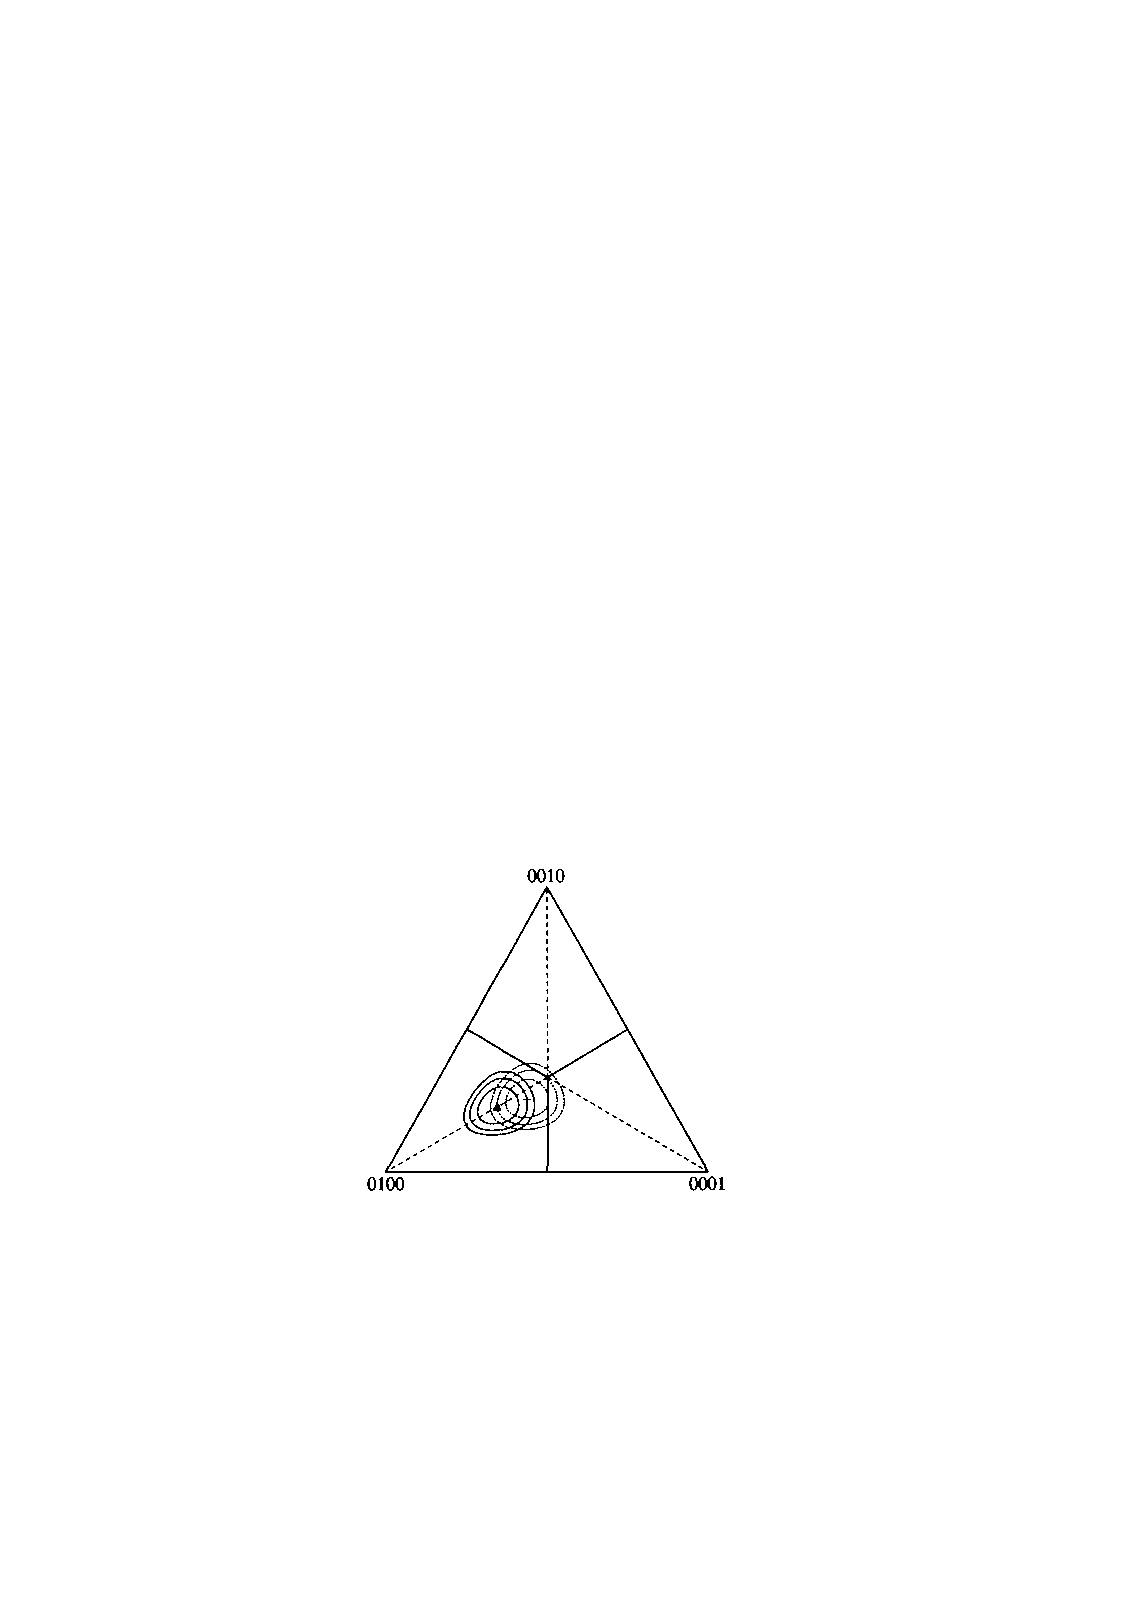
\includegraphics[scale=2]{../newimages/Newton1996Fig3.pdf}}}
	\put(40,-320){Darker ovals indicate probability contours for datasets given the truth}
	\put(60,-350){(note that repeatability $\approx$ 100\%)}
	\put(40,-380){Lighter ovals show probability contours for bootstrapping for one dataset.}
	\put(60,-410){Many real datasets will have BP much $<$ 100\%}
	\put(-40,-50){Figure 3 from \citet{Newton1996}}
\end{picture}



\myNewSlide
\large
Bootstrap proportions have been characterized as providing:
\begin{compactitem}
	\item {\color{grey} a measure of repeatability,}
	\item  {\color{grey} an estimate of the probability that the tree is correct (and criticized as being too conservative in this context),}
	\item the P-value for a tree or clade
\end{compactitem}




\myNewSlide
\section*{coin flipping (yet again)}
$N=100$ and $H=60$

Can we reject the hypothesis of a fair coin?

We can use simulation to generate the null distribution (we could actually use the binomial distribution to analytically solve this one)...

\myNewSlide

\begin{picture}(0,0)(0,0)
	\put(-10,-250){\makebox(0,0)[l]{\includegraphics[scale=1.0]{/Users/mholder/Documents/ku_teaching/BIOL-848-2010/images/nullhist.pdf}}}
	\put(180,-250){\color{red} P-value $\approx$ 0.029 }
\end{picture}

\myNewSlide
If we bootstrap we get a sense of the variability in our estimate, but we can also get a tail probability for $\Pr(p^{(boot)} \leq 0.5)$

\myNewSlide

\begin{picture}(0,0)(0,0)
	\put(-60,-250){\makebox(0,0)[l]{\includegraphics[scale=1.0]{/Users/mholder/Documents/ku_teaching/BIOL-848-2010/images/boothist.pdf}}}
	\put(60,-250){\color{red}$ \Pr(p^{(boot)} \leq 0.5)\approx$ 0.027 }
\end{picture}

\myNewSlide
\begin{picture}(-0,0)(-0,0)
	\put(60,00){\makebox(30,-150)[l]{\includegraphics[scale=0.5]{/Users/mholder/Documents/ku_teaching/BIOL-848-2010/images/nullhist.pdf}}}
	\put(60,-260){\makebox(30,-150)[l]{\includegraphics[scale=0.5]{/Users/mholder/Documents/ku_teaching/BIOL-848-2010/images/boothist.pdf}}}
\end{picture}



\includepdf[pages={28-45}]{/Users/mholder/Documents/ku_teaching/BIOL-848-2010/lec16-Bootstrapping/lec16Bootstrapping.pdf} 

\myNewSlide
\section*{\citet{EfronHH1996} view of tree space}
\begin{picture}(-0,0)(-0,0)
	\put(-10,-90){\makebox(30,-150)[l]{\includegraphics[scale=3]{/Users/mholder/Documents/ku_teaching/BIOL-848-2010/images/EfronHH-treespace-fig.pdf}}}
\end{picture}








\myNewSlide
\section*{\citet{Kim2000} view of tree space}
\begin{picture}(-0,0)(-0,0)
	\put(-10,-90){\makebox(30,-150)[l]{\includegraphics[scale=2.5]{/Users/mholder/Documents/ku_teaching/BIOL-848-2010/images/Kim-treespace.pdf}}}
\end{picture}

\myNewSlide
\section*{Parsimony-informative Pattern Frequency Space}
\begin{picture}(-0,0)(-0,0)
	\put(10,-140){\makebox(30,-150)[l]{\includegraphics[scale=1.]{/Users/mholder/Documents/ku_teaching/BIOL-848-2010/images/simple-treespace.pdf}}}
\end{picture}

\myNewSlide
\section*{Pattern Frequency Space With Observed Data}
\begin{picture}(-0,0)(-0,0)
	\put(10,-140){\makebox(30,-150)[l]{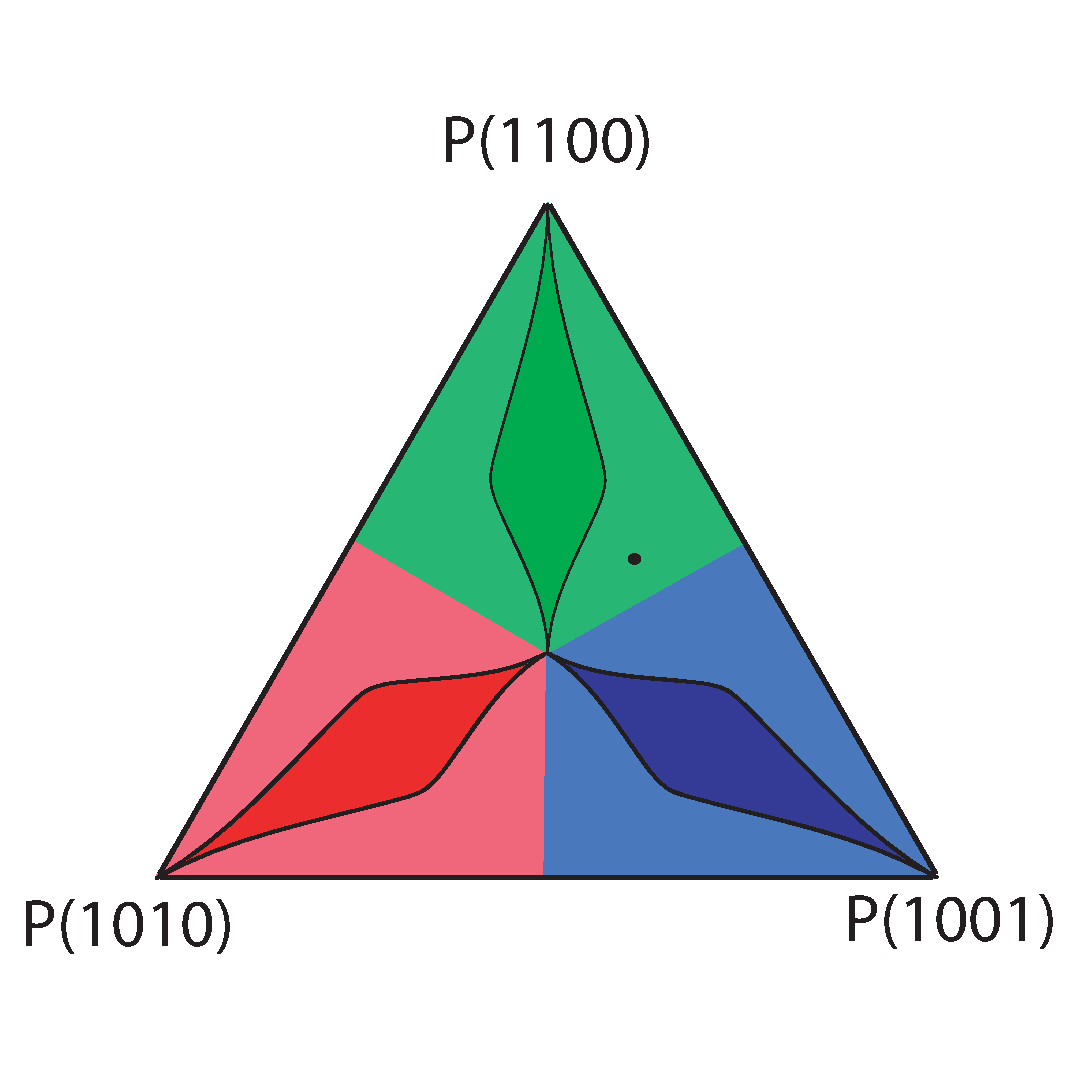
\includegraphics[scale=1.]{/Users/mholder/Documents/ku_teaching/BIOL-848-2010/images/simple-treespace-sample.pdf}}}
	\put(370,-183){$f_X$}
\end{picture}

\myNewSlide
\section*{Bootstrapping in Pattern Frequency Space}
\begin{picture}(-0,0)(-0,0)
	\put(10,-150){\makebox(30,-150)[l]{\includegraphics[scale=1.]{/Users/mholder/Documents/ku_teaching/BIOL-848-2010/images/simple-treespace-boot.pdf}}}
\end{picture}



\myNewSlide
\section*{\cite{Susko2010} aBP}
Susko reports that the curvature arguments of \citet{EfronHH1996} and \citet{Shimodaira2002}, while not incorrect, ignore the {\bf sharp point} in parameter space around the polytomy.

He uses the curvature of the likelihood function to correct bootstrap proportions so that $1-aBP$ accurately estimates the $P$-value.

You need to perform a different correction when you know the candidate tree {\em a priori} versus when you are putting BP on the ML tree.

BP may {\bf not} be conservative when you correct for selection bias.

\myNewSlide
\begin{picture}(-0,0)(-0,0)
	\put(-60,-150){\makebox(30,-150)[l]{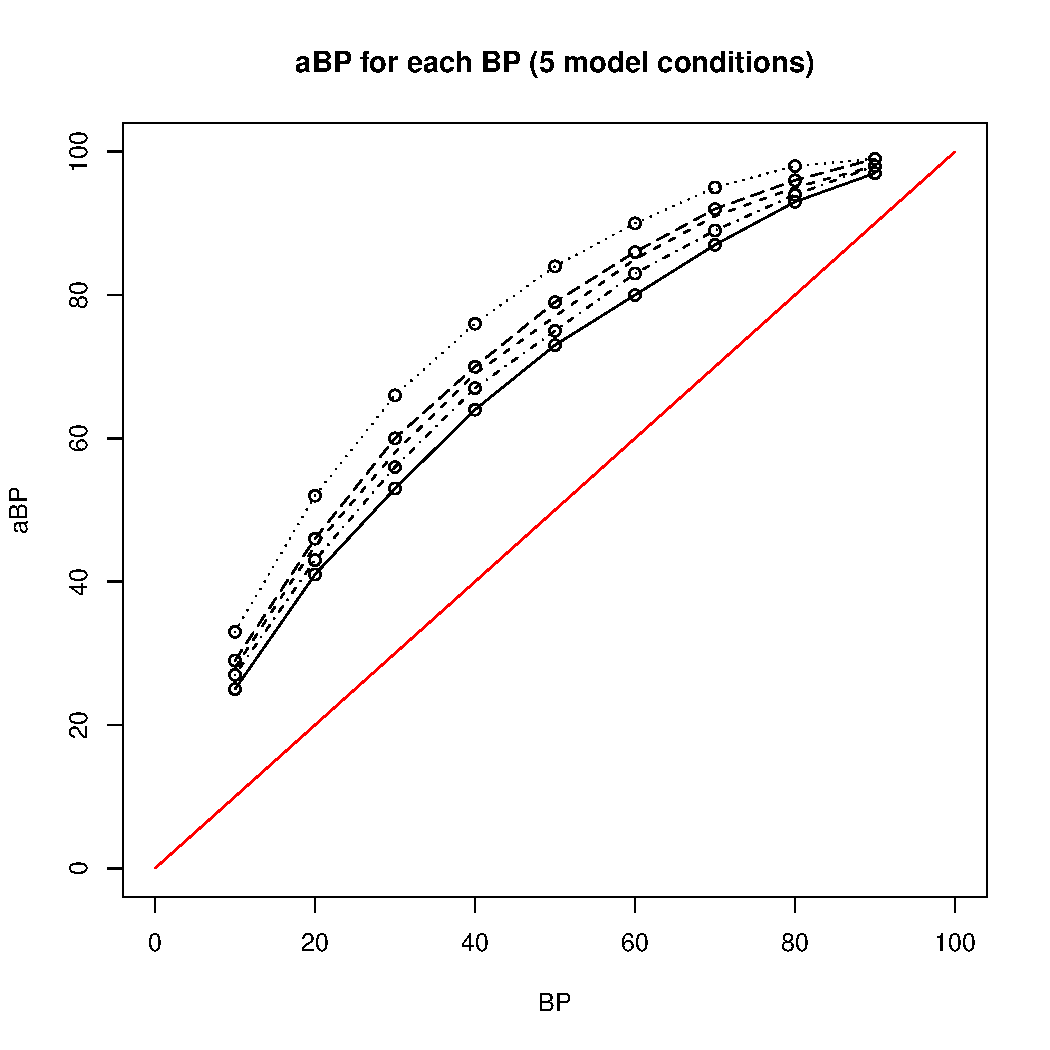
\includegraphics[scale=0.75]{../scripts/Susko2010Table3aBP.pdf}}}
	\put(300,-150){\makebox(30,-150)[l]{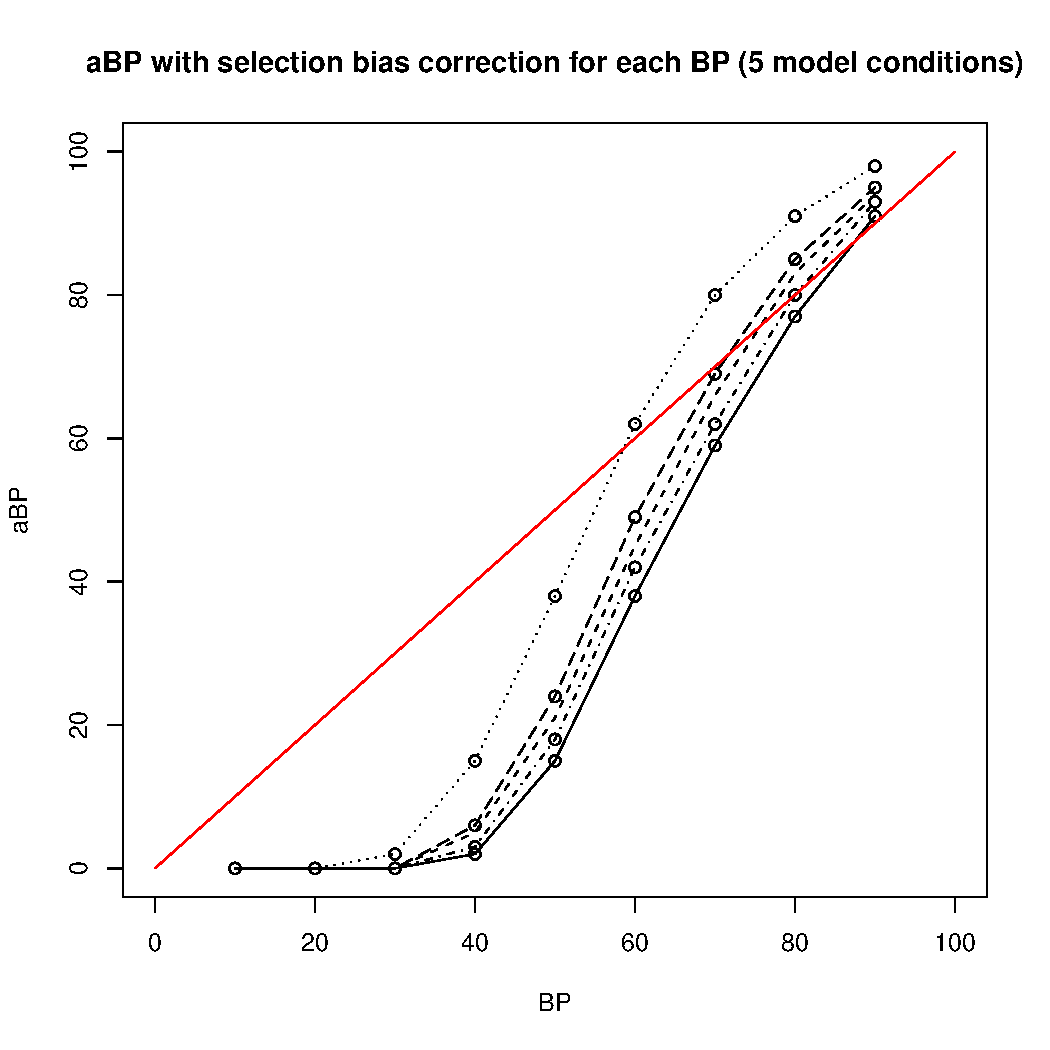
\includegraphics[scale=0.75]{../scripts/Susko2010Table3aBPMLCorrection.pdf}}}
\end{picture}


\myNewSlide
\section*{aBP in Pattern Frequency Space}
\begin{picture}(-0,0)(-0,0)
	\put(-50,-0){Null distribution for BP}
	\put(-40,-30){is calculated using}
	\put(-40,-60){Normal approximations from}
	\put(-40,-90){polytomy}
	\put(10,-150){\makebox(30,-150)[l]{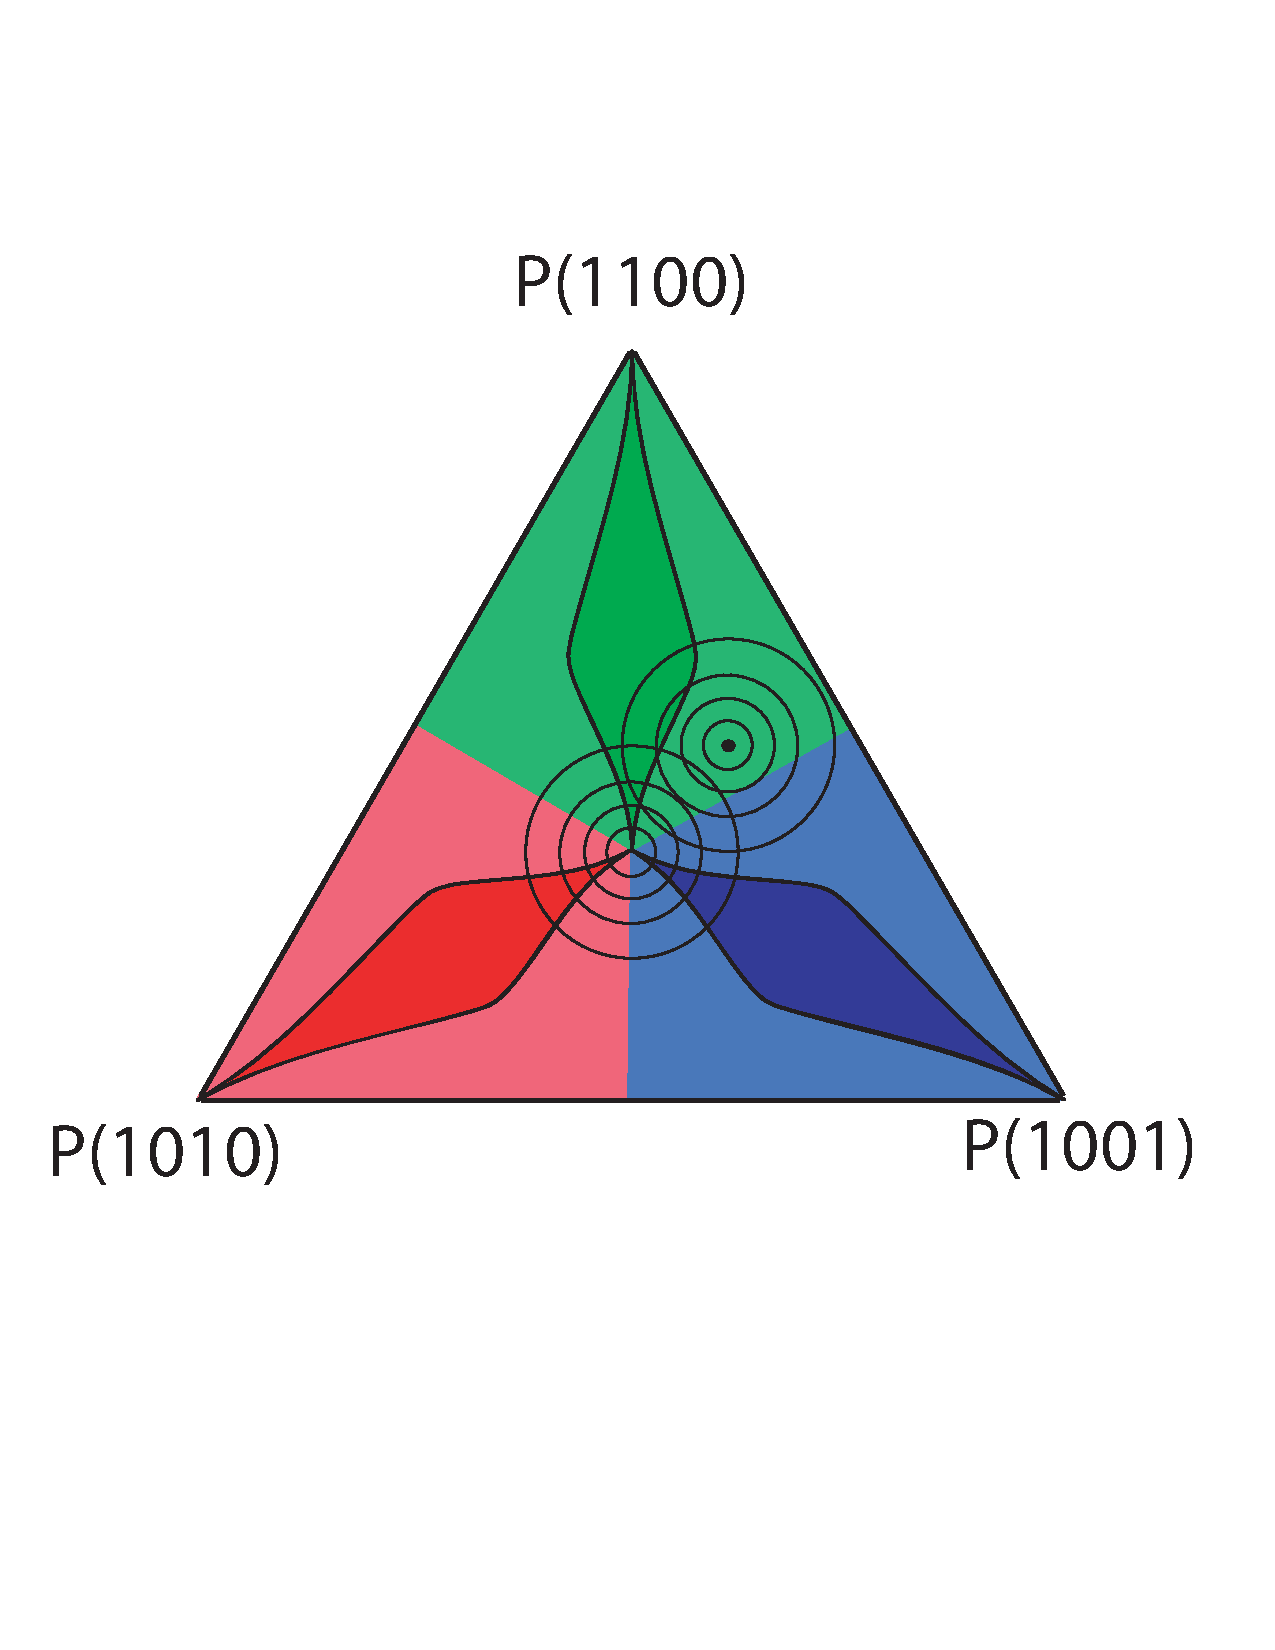
\includegraphics[scale=1.]{../newimages/simple-treespace-abp.pdf}}}
\end{picture}


\myNewSlide
\section*{ML scores in Pattern Frequency Space}
\begin{picture}(-0,0)(-0,0)
	\put(10,-120){\makebox(30,-190)[l]{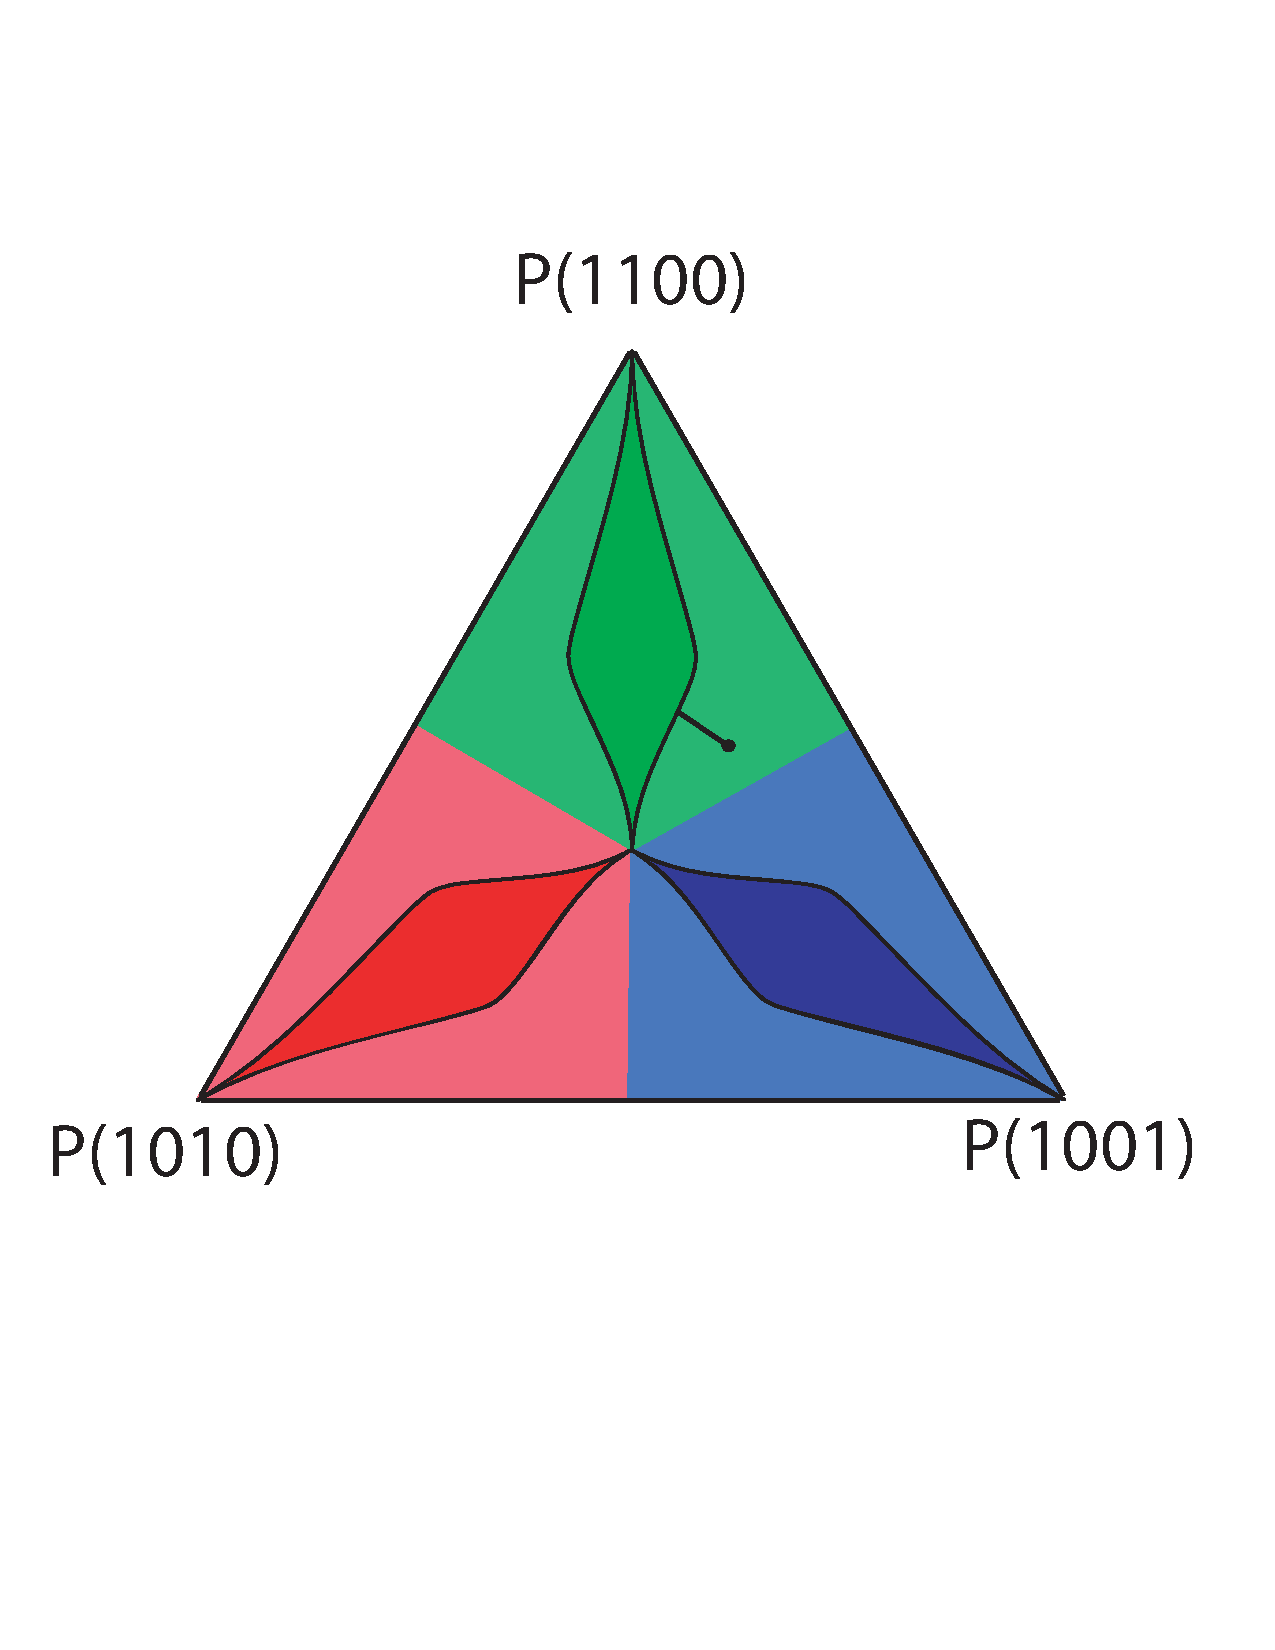
\includegraphics[scale=1.]{../newimages/simple-treespace-pp1v2.pdf}}}
	\put(-30,-0){$\ln L(T_1|X) = -D_{KL}(f_X||f_{T_1})$}
\end{picture}

\myNewSlide
\section*{Bootstrapping in Pattern Frequency Space}
\begin{picture}(-0,0)(-0,0)
	\put(10,-150){\makebox(30,-150)[l]{\includegraphics[scale=1.]{/Users/mholder/Documents/ku_teaching/BIOL-848-2010/images/simple-treespace-boot.pdf}}}
\end{picture}

\myNewSlide
\section*{Bootstrapping in Pattern Frequency Space (if you had more data)}
\begin{picture}(-0,0)(-0,0)
	\put(-50,-0){AU Test uses multiple sequence}
	\put(-40,-30){lengths to correct BP for}
	\put(-40,-60){any curvature in the boundary }
	\put(-40,-90){between trees}
	\put(10,-150){\makebox(30,-150)[l]{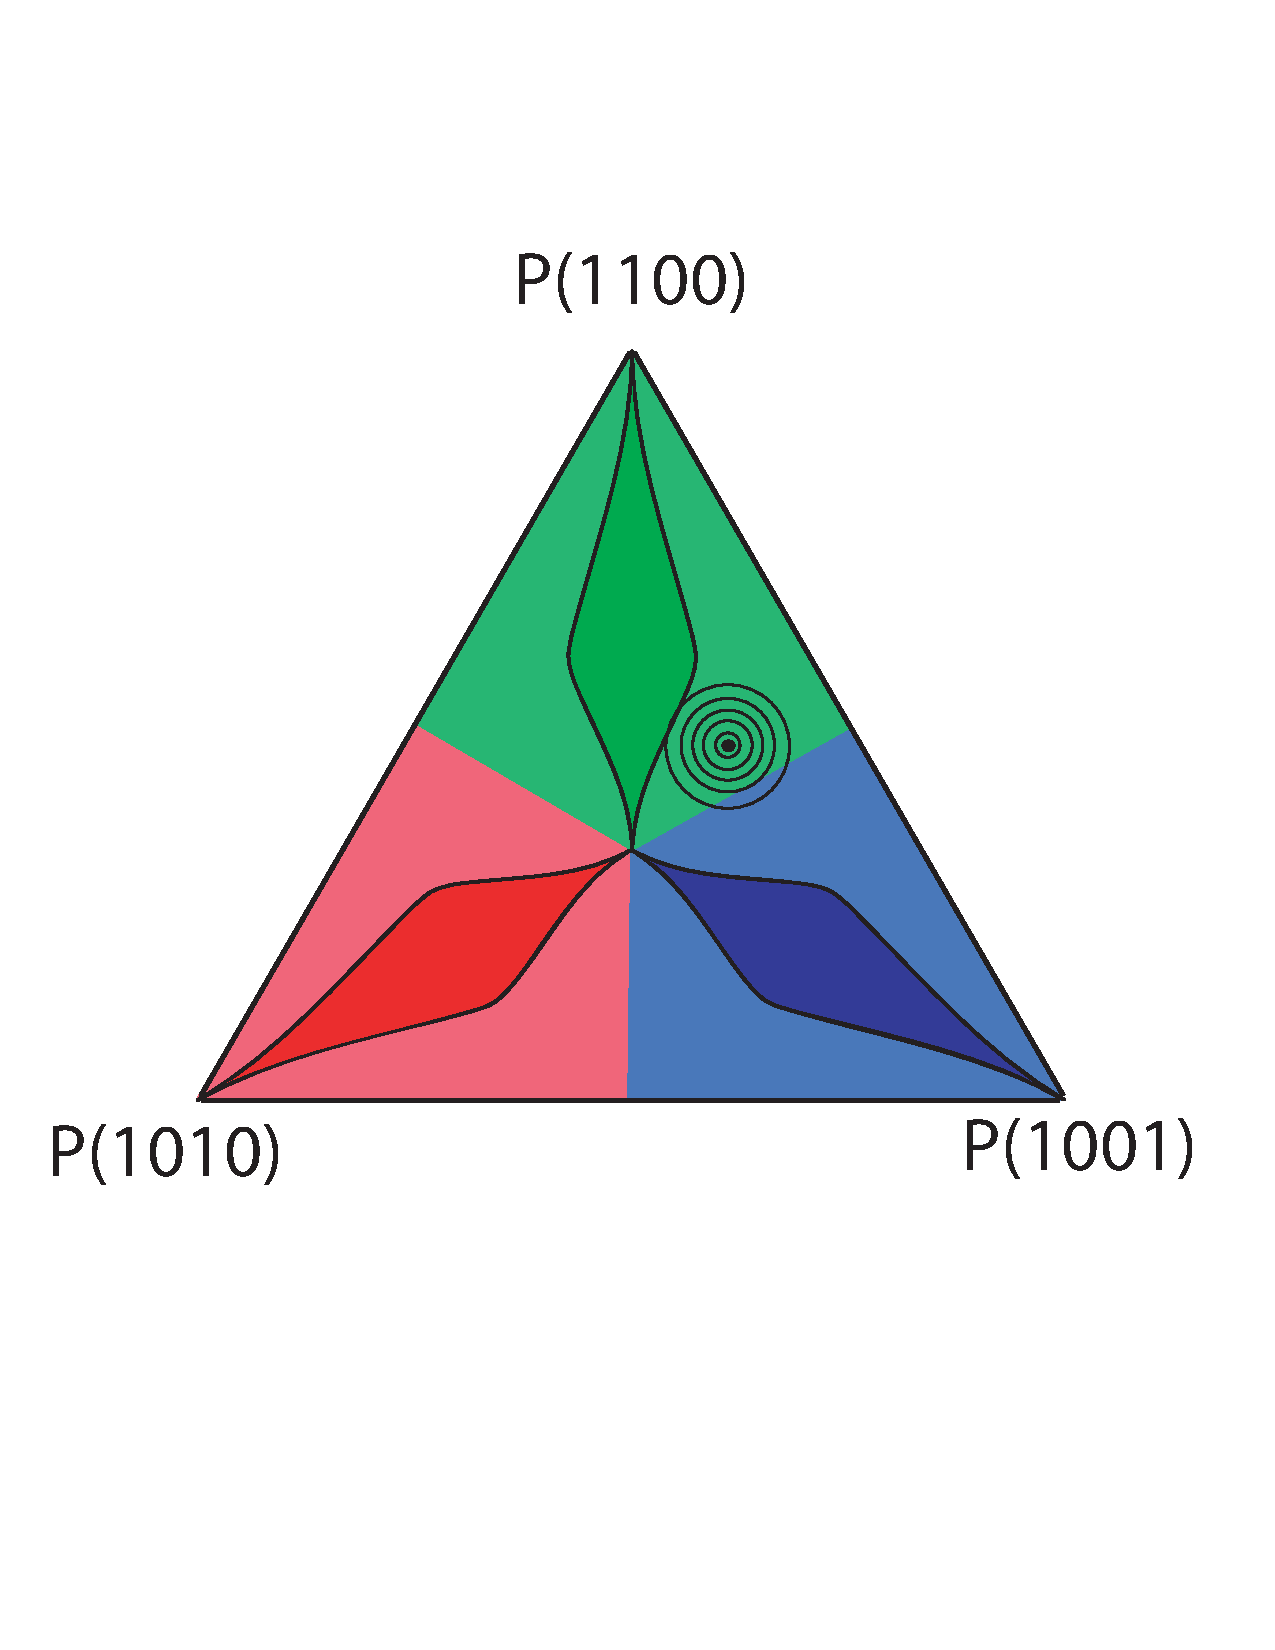
\includegraphics[scale=1.]{../newimages/simple-treespace-boot-more.pdf}}}
\end{picture}

\myNewSlide
\section*{aLRT and aBayes in Pattern Frequency Space}
\begin{picture}(-0,0)(-0,0)
	\put(10,-120){\makebox(30,-190)[l]{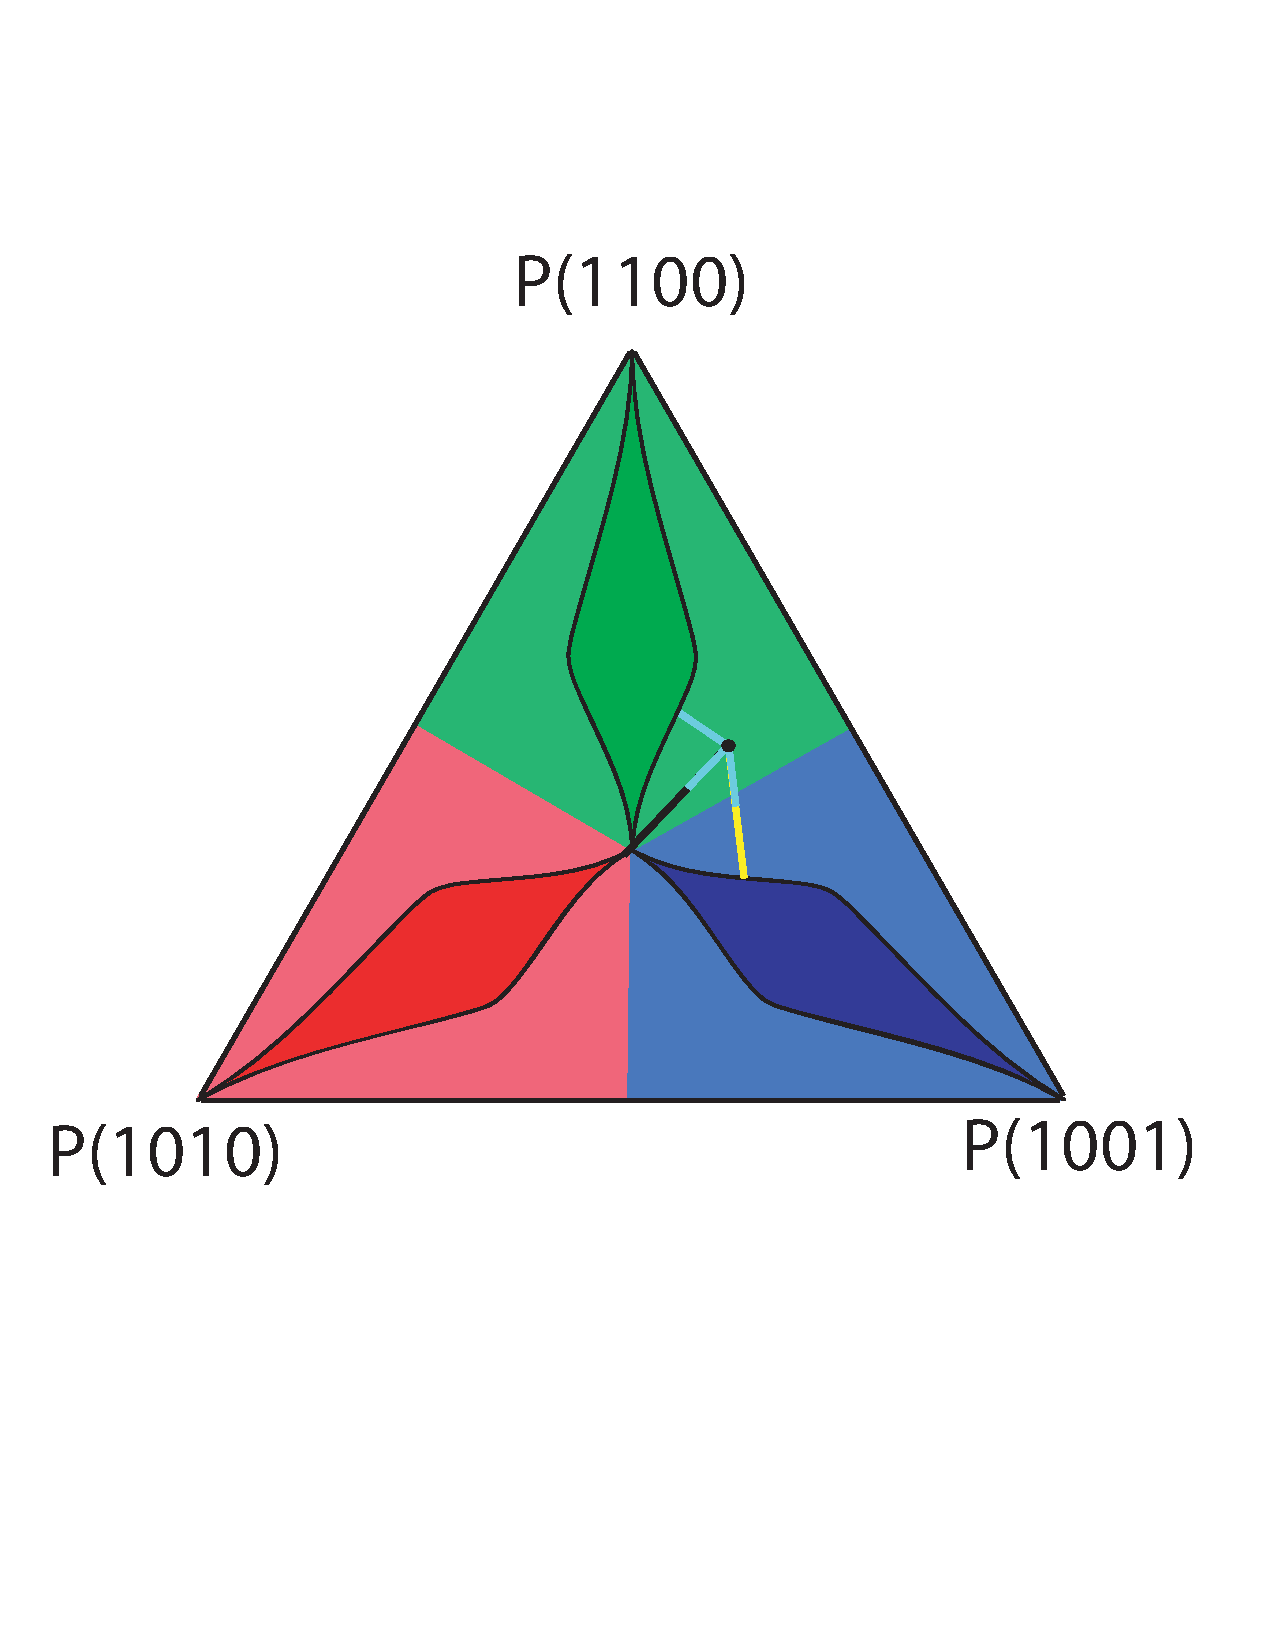
\includegraphics[scale=1.]{../newimages/simple-treespace-ppv2.pdf}}}
	\put(-50,-0){In aLRT, we use mixtures of $\chi^2$}
	\put(-40,-30){and selection bias corrections}
	\put(-40,-60){to calculate the $P$-value.}
	\put(370,-0){In aBayes, we normalize}
	\put(380,-30){the ML scores to (0,1)}
\end{picture}

\myNewSlide
\section*{KH Test in Pattern Frequency Space}
\begin{picture}(-0,0)(-0,0)
	\put(10,-120){\makebox(30,-190)[l]{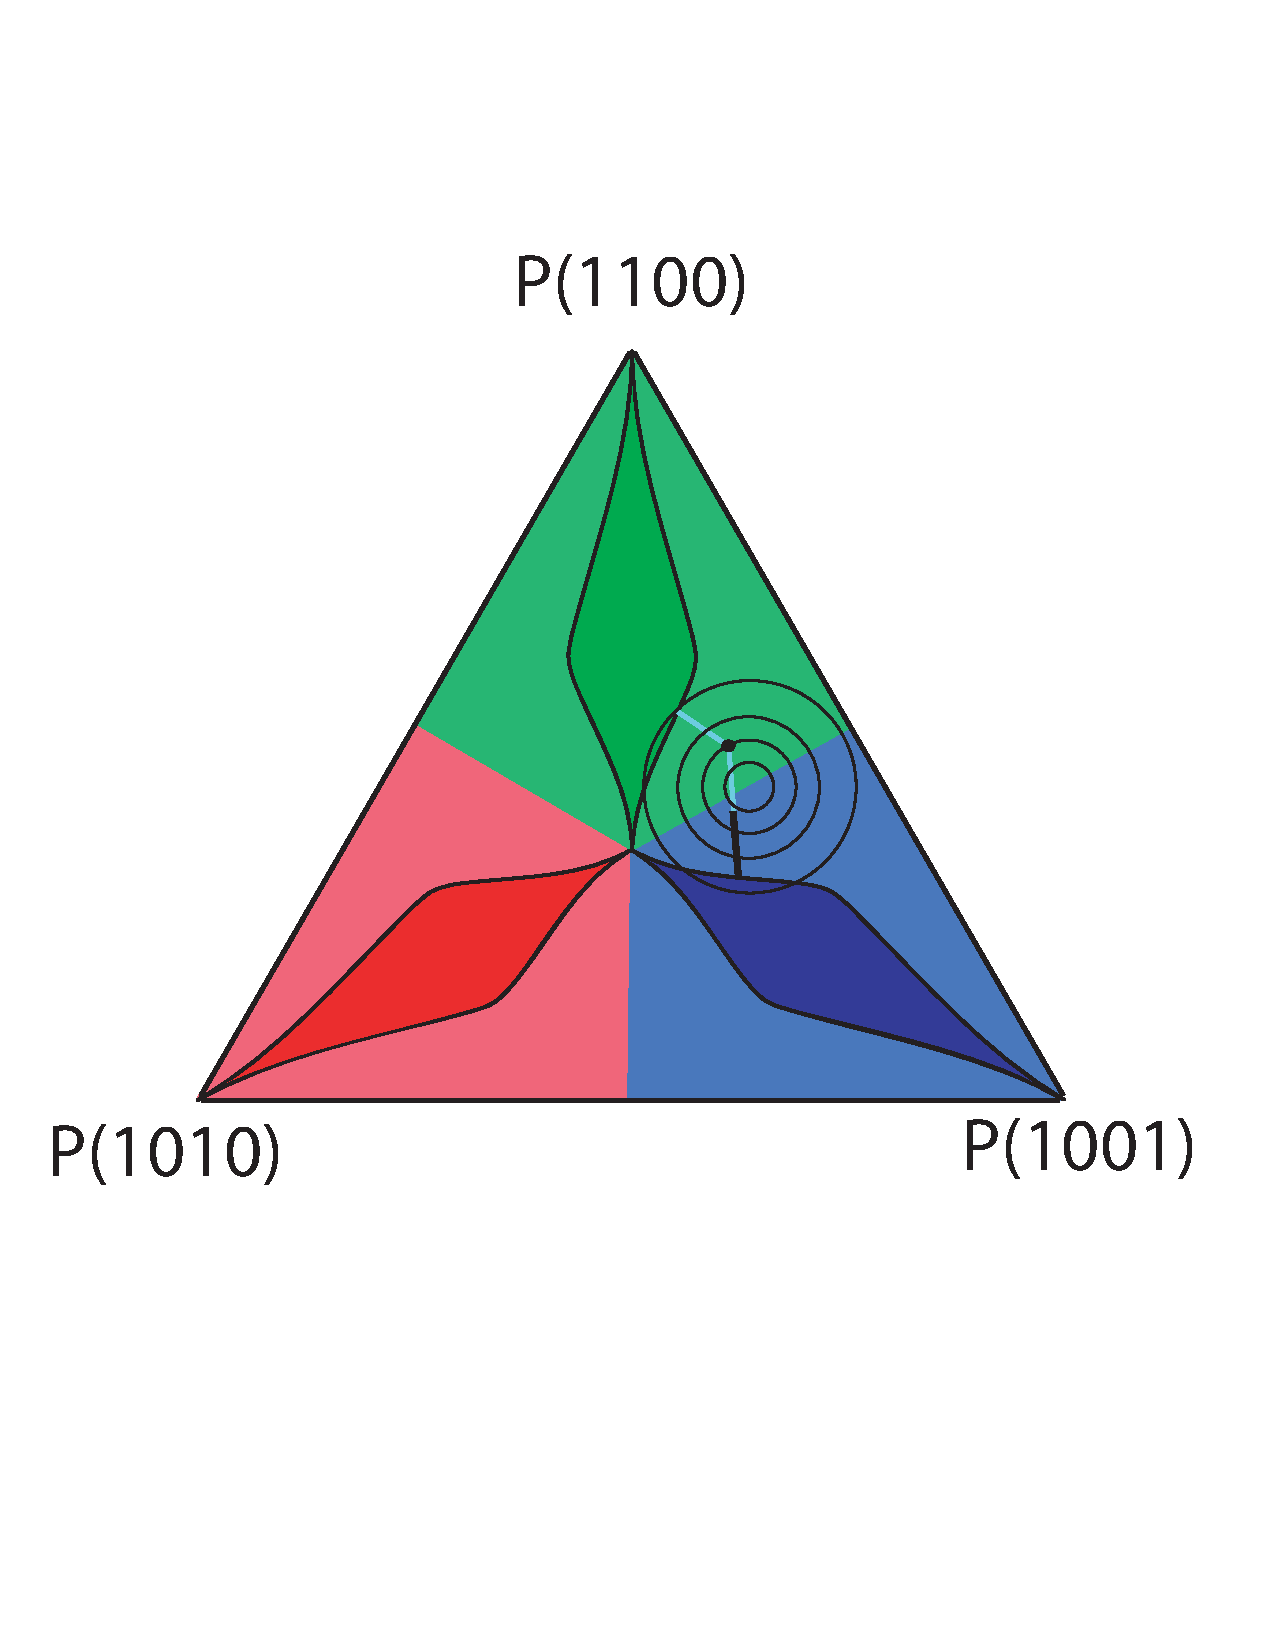
\includegraphics[scale=1.]{../newimages/simple-treespace-kh.pdf}}}
	\put(-50,-0){Uses the $\delta$ test statistic}
	\put(-40,-30){and a null distribution}
	\put(-40,-60){{\em centered} on the boundary}
\end{picture}

\myNewSlide
\section*{Parametric bootstrapping in Pattern Frequency Space}
\begin{picture}(-0,0)(-0,0)
	\put(10,-120){\makebox(30,-190)[l]{\includegraphics[scale=1.]{../newimages/simple-treespace-parametricBP.pdf}}}
	\put(-50,-0){Uses the $\delta$ test statistic}
	\put(-40,-30){and a null distribution}
	\put(-40,-60){{\em centered} on point that}
	\put(-40,-90){arises from the best}
	\put(-40,-120){tree in $H_0$}
\end{picture}


\myNewSlide
\section*{Summary - Part 1}

\begin{itemize}
	\item $\delta(T_1,T_2|X) = 2\left[\ln L(T_1|X) - \ln L(T_2|X)\right]$ is a powerful statistic for discrimination between trees.
	\item We can assess confidence by considering the variance in signal between different characters.
	\item Bootstrapping helps us assess the variance in $\ln L$ that we would expect to result from sampling error.
\end{itemize}

\myNewSlide
\section*{Summary - Part 2}
\normalsize
A (very) wide variety of tests differ by:
\begin{itemize}
	\item Null hypotheses:
	\begin{compactitem}
		\item Expected scores are the same $\rightarrow$ boundary tests. {\bf More robust ?}
		\item A tree consistent with the null is correct $\rightarrow$ tests that use the full info of the model. {\bf More powerful?}
	\end{compactitem}
	\item How to use variance information:
	\begin{compactitem}
		\item Rely on ``raw'' bootstrap variability,
		\item Invoke assumptions of normality of scores,
		\item Use $\chi^2$ variants.
	\end{compactitem}
	\item Whether or not the trees must be specified {\em a priori} -- KH Test requires the trees to be specified {\em a priori}.
\end{itemize}

\myNewSlide
\normalsize
\bibliography{phylo}
\end{document}

